\documentclass[letterpaper]{book}
\usepackage[spanish,es-noshorthands,es-tabla,es-lcroman]{babel}

\usepackage{fix-cm}
\usepackage[
  compact,
  newparttoc,
  newlinetospace,
]{titlesec}
\usepackage{titletoc}
\usepackage[strict]{changepage}

\usepackage{lipsum}% for dummy text
\usepackage[default]{lato}
\renewcommand{\mddefault}{l}

\usepackage[usenames,dvipsnames,svgnames,table]{xcolor}

\usepackage{amsmath, amsfonts, amssymb, amsthm}
\usepackage{bm}
%\usepackage{icomma} % Paquete para escribir correctamente el espacio seguido de la coma (en modo matemático)

% A mi parecer, es mejor estéticamente utilizar lo siguiente:
\AtBeginDocument{%
  \mathchardef\stdcomma=\mathcode`,
  \mathcode`,="8000
}
\begingroup\lccode`~=`, \lowercase{\endgroup\def~}{\stdcomma\,}


\usepackage{thmtools}
\usepackage{mathtools}
\usepackage{bookmark}
\usepackage{booktabs}
\usepackage{calc}
\usepackage{caption}
\usepackage{changepage}
\usepackage[inline]{enumitem}
\usepackage{tasks}
\usepackage{etoolbox}
\usepackage{fancyhdr}
\usepackage{floatrow}
\usepackage{graphicx}
\usepackage{subfig}
\usepackage{marginfix}
\usepackage{marginnote}
\usepackage{mdframed}
\usepackage{microtype}
\usepackage{multicol}
\usepackage{ragged2e}
\usepackage{cancel}
\usepackage{verbatim}

\usepackage[makeindex]{imakeidx} % Requerido para hacer un índice

\makeindex[options=-s MyStyle.ist] % Le dice a LaTeX que cree los archivos necesarios para la 'indexación'.

\usepackage{hyperref}

\usepackage{geometry} % In some weird cases, geometry might need to be loaded after hyperref
\usepackage{qrcode}
\usepackage{ccicons}


\usepackage{tikz}
\usepackage{tikz-3dplot}

\usetikzlibrary{shapes}
\usetikzlibrary{positioning}
\usetikzlibrary{shapes.geometric}
\usetikzlibrary{calendar}
\usetikzlibrary{mindmap}
\usetikzlibrary{arrows.meta}
\usetikzlibrary{calc}
\usetikzlibrary{intersections}
\usetikzlibrary{decorations.pathreplacing}
\usetikzlibrary{matrix}
\usetikzlibrary{backgrounds}
\usetikzlibrary{fit}
\usetikzlibrary{3d}
\usetikzlibrary{patterns,angles,quotes}
\usetikzlibrary{fadings}

\usepackage{pgfplots}
\pgfplotsset{compat=1.18}
\usetikzlibrary{pgfplots.fillbetween}


\geometry{
    %showframe,
	letterpaper,
    asymmetric,
	ignorefoot,
	ignorehead,
	right=7.7cm,
	left=2cm,
	top=2.5cm,
	bottom=2.5cm,
	footskip=2\baselineskip,
	footnotesep=0mm,
	marginparwidth=5cm,
	marginparsep=7mm,
	headheight=0mm,
}
%\reversemarginpar

\setlength{\parskip}{0.8\baselineskip}
%\setlength{\parindent}{0ex}
\setlength{\headheight}{12.0pt}

% Saving some length as commands
\newlength{\wholeMargin}
\setlength{\wholeMargin}{\marginparwidth}
\addtolength{\wholeMargin}{\marginparsep}

\newlength{\wholeWidth}
\setlength{\wholeWidth}{\textwidth}
\addtolength{\wholeWidth}{\wholeMargin}

\newcommand{\symmetricalPage}{
	\fancyhfoffset[L]{0mm}
	\newgeometry{
		ignorefoot,
		ignorehead,
		left=3cm,
		right=3cm,
		top=3cm,
		bottom=3cm,
		marginparwidth=0cm,
		marginparsep=0mm
	}
}
\newcommand{\asymmetricalPage}{
	\restoregeometry
}

%%%%%%

\urlstyle{rm}
\hypersetup{
	pdfborder={1 1 0},
	pdfcreator=LaTeX,
	colorlinks=true,
	linkcolor=black,
	linktoc=all,
	urlcolor=black,
	citecolor=black,
	filecolor=black,
}

\fancypagestyle{fancy}{
	\renewcommand{\headrulewidth}{0pt}
	\fancyhf{}
	\fancyhfoffset[RO]{\marginparsep + \marginparwidth}
    %\fancyhfoffset[LE]{- 0.05\marginparsep}
    \rhead[{\footnotesize\bfseries\protect\hyperref[toc-contents]{\thepage}\hspace{-1.13\marginparwidth}}]{\rightmark}
    \lhead[\leftmark]{{\footnotesize\bfseries\protect\hyperref[toc-contents]{\thepage}}}
}
\pagestyle{fancy}

\makeatletter
\def\chaptermark#1{\markboth{\protect\hyper@linkstart{link}{\@currentHref}{\textbf{\chaptertitlename~\thechapter} ~#1}\protect\hyper@linkend}{}}
\def\sectionmark#1{\markright{\protect\hyper@linkstart{link}{\@currentHref}{\textbf{\thesection} ~#1}\protect\hyper@linkend}}
\makeatother

\fancypagestyle{plain}{ % Estilo para cuando se especifica un estilo de página simple
	\fancyhead{} % Borrar encabezados
	\renewcommand{\headrulewidth}{0pt} % Eliminar línea de encabezado
}

\usepackage{emptypage} % Este paquete elimina encabezados y pies de página en páginas vacías entre capítulos. Importante para prólogos, introducción, etc.


%%%%%%%%%%%%%%%%%%%%%%%%%%%%%%%%%%%%%%%%%%%%%%%%%%%%%%%%%%%%%%%%%%%%%%%%%%%%%%%%
%		Titling
%%%%%%%%%%%%%%%%%%%%%%%%%%%%%%%%%%%%%%%%%%%%%%%%%%%%%%%%%%%%%%%%%%%%%%%%%%%%%%%%

\newlength{\subtitleRubberWidth}\setlength{\subtitleRubberWidth}{2cm}
\newlength{\subtitleDefaultPadding}\setlength{\subtitleDefaultPadding}{2mm}
\newlength{\subtitleRubberHeight}\setlength{\subtitleRubberHeight}{4.5cm}
\titleformat{\chapter}[block]
{} % format
{%
	\begin{tikzpicture}%
		\node [font=\fontsize{1cm}{1.2cm}\selectfont\bfseries] (chapterLabel) {\hspace{-.3ex}\chaptername};
		\draw [xshift=-2mm, black, ultra thick] (chapterLabel.south west) -- (chapterLabel.south east);
	\end{tikzpicture}
	\begin{tikzpicture}[remember picture, overlay, inner sep=0mm]
%		Coordinates
		\coordinate[xshift=-1in-\evensidemargin-\subtitleRubberWidth] (rubberNorthWest) at (current page.north east);
		\coordinate[xshift=\subtitleRubberWidth, yshift=-\subtitleRubberHeight] (rubberSouthEast) at (rubberNorthWest);
		\coordinate[yshift=-\subtitleRubberHeight] (rubberSouthWest) at (rubberNorthWest);
		\coordinate[xshift=\subtitleDefaultPadding, yshift=-1in-\voffset-\topmargin-\headheight-\headsep] (rubberTextNorthWest) at (rubberNorthWest);
%		Drawing the rubber
		\fill[black] (rubberNorthWest) rectangle (rubberSouthEast) -- +(-\subtitleRubberWidth/2, -8mm) -- (rubberSouthWest) -- cycle;
		\draw[white] (rubberSouthWest)[xshift=\subtitleRubberWidth/2] node [
			anchor=south,
			align=center,
			text width=\subtitleRubberWidth-2\subtitleDefaultPadding
		] {
			%\chapterNumberFont
            \fontsize{2cm}{2.4cm}\selectfont
			\color{White}
			\thechapter\startcontents
		};
	\end{tikzpicture}%
}
{0pt} % sep
{% code before
	\blockmargin%
	\begin{adjustwidth}{0mm}{-\wholeMargin}
		\FlushLeft
		\begingroup
		%\chapterFont
        \fontsize{1.5cm}{1.8cm}\selectfont\raggedright\bfseries%
		\noHyphen%
}[ % code after
		\endgroup
	\end{adjustwidth}
	\unblockmargin%
]

\titleformat{name=\chapter, numberless}[block]
{} % format
{}
{0pt} % sep
{ % code before
	\begin{adjustwidth}{0mm}{-\wholeMargin}
		\FlushLeft
		\begingroup
		%\chapterFont
        \fontsize{1.5cm}{1.8cm}\selectfont\raggedright\bfseries%
		\noHyphen%
	}[ % code after
	\endgroup
\end{adjustwidth}
]

\titlespacing*% the star makes the first paragraph after the title unindented
    {\chapter}% command to format
    {0pt}% spacing on left
    {0.13\textheight}% spacing before title
    {4ex}% spacing after the title
    [0pt]% extra margin on the right

%-----------------------------------------------------------------------------
%   TABLA DE CONTENIDOS
%-----------------------------------------------------------------------------

\contentsmargin{0cm}

% Estilo de texto de parte
\titlecontents{part}[0cm]
{\addvspace{20pt}\centering\large\bfseries\color{white}}
{}
{}
{}

% Estilo de texto de capítulo
\titlecontents{chapter}[1.4cm] % Sangría
{\addvspace{12pt}\large\bfseries} % Opciones de espaciado y fuente para los capítulos
{\contentslabel[\Large\thecontentslabel]{1cm}} % Número de capítulo
{}
{\normalsize\;\titlerule*[.8pc]{.}\;\thecontentspage} % Número de página

% Estilo de texto de sección 
\titlecontents{section}[2.4cm] % Sangría
{\addvspace{3pt}} % Opciones de espaciado y fuente para las secciones
{\contentslabel[\thecontentslabel]{1cm}} % Número de sección
{}
{\normalsize\;\titlerule*[.8pc]{.}\;\thecontentspage} % Número de página
[]

% Estilo de texto de subsección 
\titlecontents{subsection}[3.4cm] % Sangría
{\addvspace{2pt}\small} % Opciones de espaciado y fuente para las secciones
{\contentslabel[\thecontentslabel]{1cm}} % Número de subsección
{}
{\ \titlerule*[.8pc]{.}\;\thecontentspage} % Número de página
[]

\pgfkeys{
	/yMarginDesign/.cd,
	alignment/.code = \RaggedRight,
	emph color/.initial = black,
	text color/.initial = black,
	size/.code = \footnotesize,
	titleFormat/.code = \bfseries\scshape,
	marginparskip/.initial = 3mm,
}

%%%%%%%%%%%%%%%%%%%%%%%%%%%%%%%%%%%%%%%%%%%%%%%%%%%%%%%%%%%%%%%%%%%%%%%%%%%%%%%%
%		Margin Paragraphs
%%%%%%%%%%%%%%%%%%%%%%%%%%%%%%%%%%%%%%%%%%%%%%%%%%%%%%%%%%%%%%%%%%%%%%%%%%%%%%%%

\makeatletter
% Typeset a paragraph in the margin
\DeclareDocumentCommand{\marginElement}{m}{%
	\marginpar{{%
			\pgfkeys{/yMarginDesign/alignment}%
			\pgfkeys{/yMarginDesign/size}%
			\color{\pgfkeysvalueof{/yMarginDesign/text color}}
      \setlist{
        noitemsep,
        left=0mm,
      }%
      #1\par\vspace*{\baselineskip}%
	}}\unskip%
}%

\newcounter{marginnote}

% Typeset a paragraph in the margin with a number (as a footnote) 
\DeclareDocumentCommand{\marginNote}{m}{%
  \stepcounter{marginnote}%
  \hyper@anchor{from-\theHmarginnote}%
  {%
    \bfseries%
    \hyper@link{}{to-\theHmarginnote}{\textsuperscript{\textcolor{\pgfkeysvalueof{/yMarginDesign/emph color}}{\themarginnote}}}%
  }%
	\marginElement{%
	  \hyper@anchor{to-\theHmarginnote}%
	  {%
	    \bfseries%
      \hyper@link{}{from-\theHmarginnote}{\textcolor{\pgfkeysvalueof{/yMarginDesign/emph color}}{\themarginnote.}}~%
	  }%
	  \ignorespaces%
		#1%
	}%
}%

% Typeset a paragraph in the margin exactly at the exact position where the command is called
\DeclareDocumentCommand{\forcedMarginElement}{m}{%
  \marginnote{{%
    \pgfkeys{/yMarginDesign/alignment}%
    \pgfkeys{/yMarginDesign/size}%
    \color{\pgfkeysvalueof{/yMarginDesign/text color}}
		#1%
  }}%
}

% Typeset a paragraph in the margin exactly at the exact position where the command is called with a number (as a footnote)
\DeclareDocumentCommand{\forcedMarginNote}{m}{%
	\printMarginNoteMark
	\ignorespaces%
	\forcedMarginElement{%
		\sideMark[#1]{\thefootnote}%
		\ignorespaces%
		#1%
	}%
}

\DeclareDocumentCommand{\sideTable}{o m}{%
	\marginpar{%
		\strictpagechecktrue%
		\checkoddpage%
		\ifoddpage%
		\justifying\footnotesize%
		\else%
		\RaggedLeft\footnotesize%
		\fi%
		\@afterindentfalse\@afterheading
		\vspace*{6mm} % compensate the table space added above the first line by the gape command
		#2
		\captionsetup*[table]{font={footnotesize},hypcap=false}
		\IfValueT{#1}{\captionof{table}{#1}}
	}
}

\DeclareDocumentCommand{\sideFigure}{o m}{%
	\marginElement{%
		\strictpagechecktrue
		\checkoddpage
		\ifoddpage%
		\RaggedRight%
		\else%
		\RaggedLeft%
		\fi%
		\@afterindentfalse\@afterheading%
		#2%
		\captionsetup*[figure]{font={footnotesize},hypcap=false}%
		\IfValueT{#1}{\vspace*{-2mm}\captionof{figure}{#1}}
	}
}

\newcommand{\noHyphen}{%
  \righthyphenmin=62
  \lefthyphenmin=62
}

\DeclareDocumentCommand{\yTitle}{m}{%
  \begingroup%
    \large\scshape\bfseries%
    #1%
  \endgroup%
}

\DeclareDocumentCommand{\printchaptertableofcontents}{}{%
  \marginElement{%
    {%
      %\vspace*{9mm}
      \yTitle{Contenido}\\[2mm]
      \printcontents{c}{1}[1]{\hypersetup{linkcolor=black}}%
    }%
  } 
}

\titlecontents{csection}
  [8mm] % Left indent
  {} % Above code
  {\contentslabel[\bfseries\thecontentslabel]{8mm}\noHyphen} % Numbered entry
  {\hspace*{-6mm}\noHyphen} % Numberless entry
  {,\hspace*{1ex}\mbox{\emph{p.~\thecontentspage}}} % Filler

%------------------------------------------------------------------------------
%   TÍTULOS DE PARTE
%------------------------------------------------------------------------------

% parte numerada en la tabla de contenido
\newcommand{\@mypartnumtocformat}[2]{%
\setlength\fboxsep{0pt}%
\noindent\colorbox{black!20}{\strut\parbox[c][.8cm]{\ecart}{\color{black!70}\Large\bfseries\centering#1}}\hskip\esp\colorbox{black}{\strut\parbox[c][.8cm]{\linewidth-\ecart-\esp}{\Large\centering#2}}}%
%%%%%%%%%%%%%%%%%%%%%%%%%%%%%%%

% parte no numerada en la tabla de contenido
\newcommand{\@myparttocformat}[1]{%
\setlength\fboxsep{0pt}%
\noindent\colorbox{black!40}{\strut\parbox[c][.8cm]{\linewidth}{\Large\centering#1}}}%
%%%%%%%%%%%%%%%%%%%%%%%%%%%%%%%

\newlength\esp
\setlength\esp{4pt}
\newlength\ecart
\setlength\ecart{1.2cm-\esp}
\newcommand{\thepartimage}{}%
\newcommand{\partimage}[1]{\renewcommand{\thepartimage}{#1}}%
\def\@part[#1]#2{%
\ifnum \c@secnumdepth >-2\relax%
\refstepcounter{part}%
\addcontentsline{toc}{part}{\texorpdfstring{\protect\@mypartnumtocformat{\thepart}{#1}}{\partname~\thepart\ ---\ #1}}
\else%
\addcontentsline{toc}{part}{\texorpdfstring{\protect\@myparttocformat{#1}}{#1}}%
\fi%
\startcontents%
\markboth{}{}%
{\thispagestyle{empty}%
\begin{tikzpicture}[remember picture,overlay]%
\node at (current page.north west){\begin{tikzpicture}[remember picture,overlay]%   
\fill[gray!20](0cm,0cm) rectangle (\paperwidth,-\paperheight);
\node[anchor=north west,inner sep=0pt,xshift=\Gm@lmargin/3,yshift=-3cm] at (current page.north west){\color{black}\scalebox{20}{\bfseries\@Roman\c@part}};
\node[anchor=south east] at (\paperwidth-1cm,-\paperheight+1cm){\parbox[t][][t]{12cm}{
\printcontents{l}{0}{\setcounter{tocdepth}{0}}%
}};
\node[anchor=north east] at (\paperwidth-1.5cm,-3.25cm){\parbox[t][][t]{15cm}{\strut\raggedleft\color{black}\fontsize{45}{45}\bfseries#2}};
\end{tikzpicture}};
\end{tikzpicture}}%
\@endpart}
\def\@spart#1{%
\startcontents%
\phantomsection
{\thispagestyle{empty}%
\begin{tikzpicture}[remember picture,overlay]%
\node at (current page.north west){\begin{tikzpicture}[remember picture,overlay]%   
\fill[gray!60](0cm,0cm) rectangle (\paperwidth,-\paperheight);
\node[anchor=north east] at (\paperwidth-1.75cm,-3.25cm){\parbox[t][][t]{15cm}{\strut\raggedleft\color{white}\fontsize{45}{45}\bfseries#1}};
\end{tikzpicture}};
\end{tikzpicture}}
\addcontentsline{toc}{part}{\texorpdfstring{%
\setlength\fboxsep{0pt}%
\noindent\protect\colorbox{gray!40}{\strut\protect\parbox[c][.7cm]{\linewidth}{\Large\protect\centering #1\quad\mbox{}}}}{#1}}%
\@endpart}
\def\@endpart{\vfil\newpage
\if@twoside
\if@openright
\null
\thispagestyle{empty}%
\newpage
\fi
\fi
\if@tempswa
\twocolumn
\fi}

\makeatother

%%%%%%%%%%%%%%%%%%%%%%%%%%%%%%%%%%%%%%%%%%%%%%%%%%%%%%%%%%%%%%%%%%%%%%%%%%%%%%%%
%		Floats
%%%%%%%%%%%%%%%%%%%%%%%%%%%%%%%%%%%%%%%%%%%%%%%%%%%%%%%%%%%%%%%%%%%%%%%%%%%%%%%%

\DeclareDocumentCommand{\isOddPage}{mm}{%
	\strictpagechecktrue%
	\checkoddpage%
	\ifoddpage%
	#1%
	\else%
	#2%
	\fi%
}

\DeclareCaptionFont{myCaptionFont}{\scshape\bfseries}
\DeclareCaptionLabelSeparator{myCaptionLabelSeparator}{\hspace*{1ex}}
\captionsetup{
  labelfont=myCaptionFont,
  justification=RaggedRight,
  labelsep=myCaptionLabelSeparator,
}

\DeclareFloatVCode{parskip}{{\vspace{\parskip}}}
\newlength{\twoparskip}
\setlength{\twoparskip}{1.5\parskip}
\DeclareFloatVCode{twoparskip}{{\vspace\twoparskip}}
\DeclareFloatSeparators{marginparsep}{\hspace\marginparsep}
\floatsetup[figure]{
    %precode=twoparskip,
    margins=hangright,
    floatwidth=\textwidth,
    font={normalsize},
    capposition=beside,
    captionskip=0mm,
    capbesideposition={top,right},
    capbesidewidth=sidefil,
    capbesidesep=marginparsep,%
    footposition=caption,
    footskip=0.5\baselineskip,
    footfont={small},
	%postcode=twoparskip,
}

\floatsetup[widefloat]{%
	capposition=bottom,
	captionskip=\baselineskip,
}



%%%%%%%%%%%%%%%%%%%%%%%%%%%%%%%%%%%%%%%%%%%%%%%%%%%%%%%%%%%%%%%%%%%%%%%%%%%%%%%%
%		Enumitem
%%%%%%%%%%%%%%%%%%%%%%%%%%%%%%%%%%%%%%%%%%%%%%%%%%%%%%%%%%%%%%%%%%%%%%%%%%%%%%%%

\setlist{
  topsep=0mm,
}
\setlist[description]{font=\scshape}
\setlist[enumerate]{font=\bfseries}
\setlist[itemize]{label={$\bullet$}}

\settasks{
    label-format = \bfseries,
    item-indent = 0.94cm,
}

%%%% MATEMÁTICAS %%%%%

\newtheoremstyle{myplain}
  {1.2\topsep}   % ABOVESPACE
  {1.2\topsep}   % BELOWSPACE
  {}  % BODYFONT
  {0pt}       % INDENT (empty value is the same as 0pt)
  {\bfseries} % HEADFONT
  {:}         % HEADPUNCT
  {5pt plus 1pt minus 1pt} % HEADSPACE
  {\thmname{#1}\thmnumber{ #2}\thmnote{ (#3)}}%                                     % Theorem head spec (can be left empty, meaning `normal')

\theoremstyle{myplain}

\newtheorem{theorem}{Teorema}[section]
\newtheorem{axiom}{Axioma}[section]
\newtheorem{lemma}{Lema}[section]
\newtheorem{proposition}{Proposición}[section]
\newtheorem{corollary}{Corolario}[section]
\newtheorem{definition}{Definición}[section]
\newtheorem*{example}{Ejemplo}
\newtheorem*{examples}{Ejemplos}
\newtheorem*{observation}{Observación}%[section]
\newtheorem*{remark}{Nota}
\newtheorem*{notation}{Notación}
\newtheorem*{commentary}{Comentario}
\newtheorem*{convention}{Convención}
\newtheorem{problem}{Problema}
\newtheorem*{Problem}{Problema}
\newtheorem*{reminder}{Recordatorio}

\newcommand{\demostracion}{\noindent\textbf{Demostración: }}

\newcommand{\solucion}{\noindent\textbf{Solución: }}

% number sets
\newcommand{\RR}[1][]{\ensuremath{\ifstrempty{#1}{\mathbb{R}}{\mathbb{R}^{#1}}}}
\newcommand{\NN}[1][]{\ensuremath{\ifstrempty{#1}{\mathbb{N}}{\mathbb{N}^{#1}}}}
\newcommand{\ZZ}[1][]{\ensuremath{\ifstrempty{#1}{\mathbb{Z}}{\mathbb{Z}^{#1}}}}
\newcommand{\QQ}[1][]{\ensuremath{\ifstrempty{#1}{\mathbb{Q}}{\mathbb{Q}^{#1}}}}
\newcommand{\CC}[1][]{\ensuremath{\ifstrempty{#1}{\mathbb{C}}{\mathbb{C}^{#1}}}}
\newcommand{\PP}[1][]{\ensuremath{\ifstrempty{#1}{\mathbb{P}}{\mathbb{P}^{#1}}}}
\newcommand{\HH}[1][]{\ensuremath{\ifstrempty{#1}{\mathbb{H}}{\mathbb{H}^{#1}}}}

\makeatletter
\def\smallunderbrace#1{\mathop{\vtop{\m@th\ialign{##\crcr
   $\hfil\displaystyle{#1}\hfil$\crcr
   \noalign{\kern3\p@\nointerlineskip}%
   \tiny\upbracefill\crcr\noalign{\kern3\p@}}}}\limits}
\makeatother

\begin{document}

\renewcommand{\theequation}{\thesection.\arabic{equation}} 

\pagestyle{empty}

\begin{titlepage}
  \symmetricalPage%
  \begingroup%
    %\tikzset{external/export=false}%%
    \begin{tikzpicture}[
        overlay,
        remember picture,
      ]
      \node[anchor=center] at ($(current page)+(-3.1,-5)$) {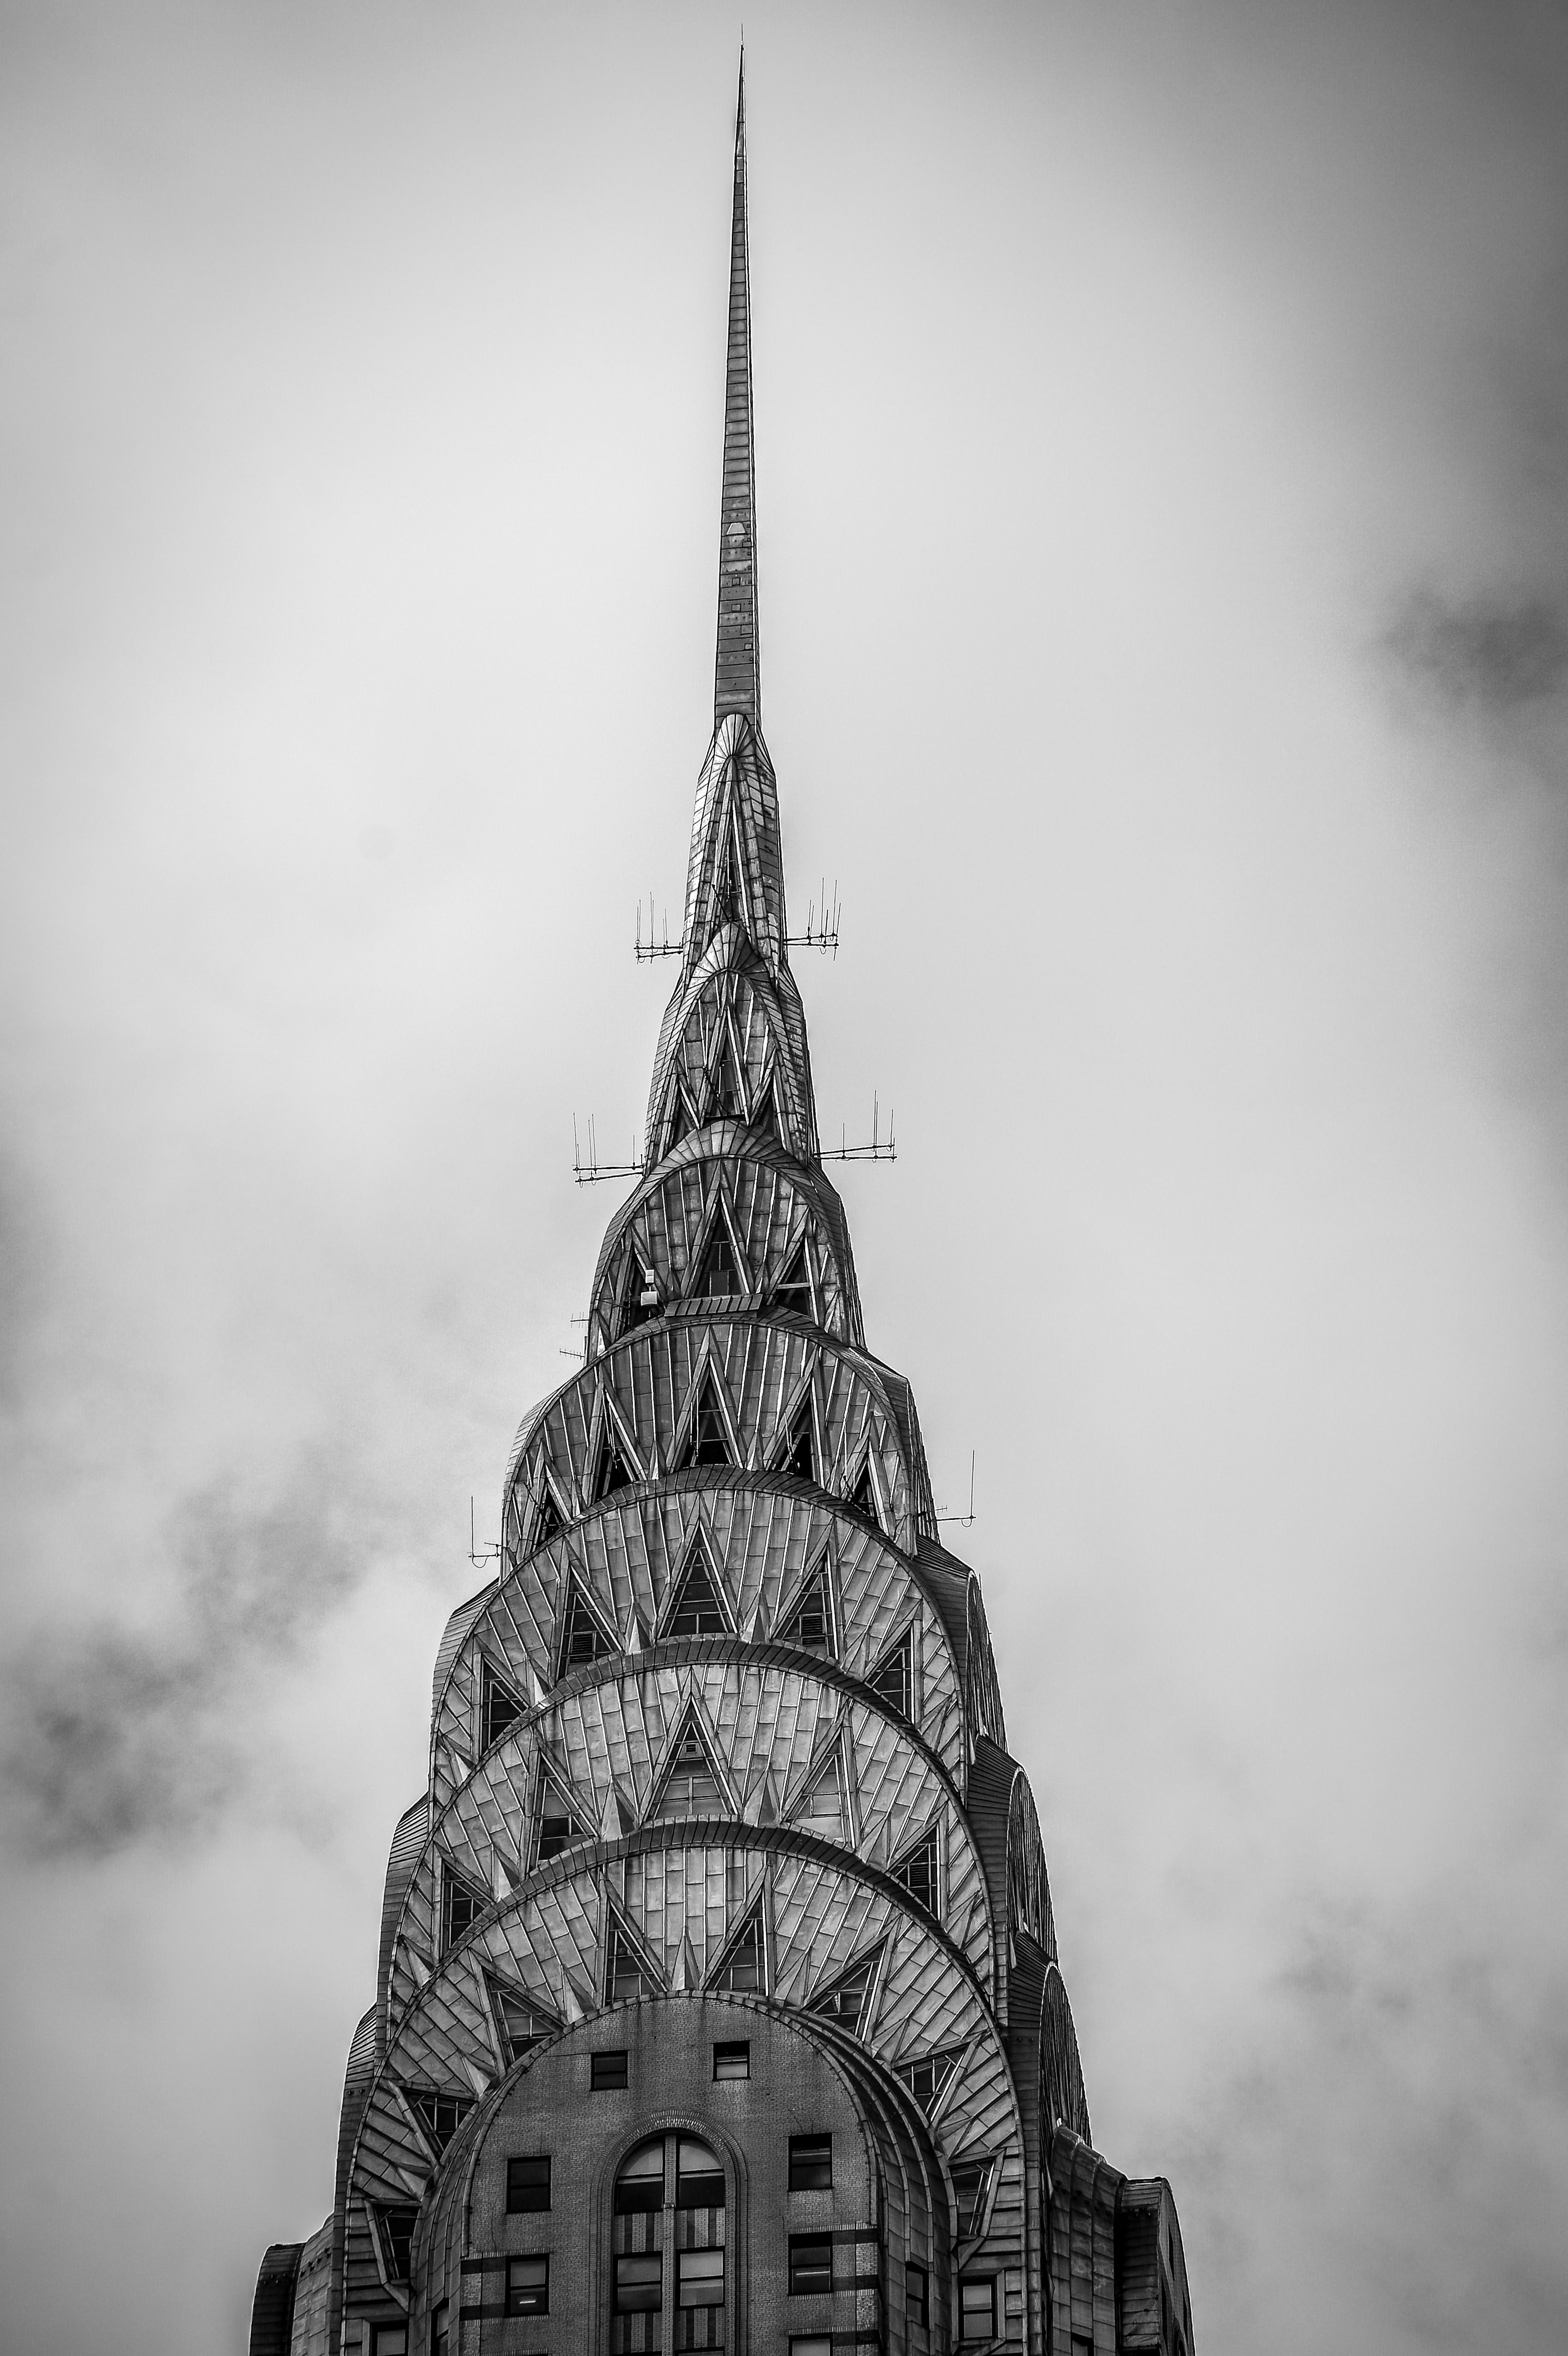
\includegraphics[width=1.3\paperwidth]{Images/Portada/FONDO.jpg}};
    \end{tikzpicture}
  \endgroup%
  %\sffamily%

  \vspace*{2cm}%
  \begingroup%
    \bfseries\flushright%
    % \scshape%
    \begingroup%
      \Huge%
      \color{black}
      \noindent\scalebox{2}{NOTAS DE}\\[10mm]
      \scalebox{2}{CÁLCULO III}\\[50mm]
    \endgroup%
    \begingroup%
      \bfseries\LARGE%
      \color{black}%
      ~\hfill\begin{tabular}{r}
          Sabino D. Castro\\[4mm]
          Antonio M. Mendoza
      \end{tabular}
      %~\hfill Sabino D. Castro\\[4mm]
      %~\hfill Antonio M. Mendoza
    \endgroup%
  \endgroup%

  \vfill%
  \noindent\parbox[b]{\linewidth-5cm}{%
    \begingroup%
      ~
    \endgroup%
  }%
  ~\hfill%
  \parbox[b]{3cm}{%
    
\includegraphics[width=\linewidth]{Images/Portada/LOGO.pdf}
  }
\end{titlepage}
\restoregeometry%

\newpage
\,

\newpage

\symmetricalPage%

\begin{tikzpicture}[remember picture,overlay]%
      \coordinate (A) at ($(current page.north)!.4!(current page.north east)$);
      \coordinate (B) at (current page.east);
      \coordinate (C) at (current page.north east);

      \filldraw[black] (A) -- (B) -- (C) -- cycle;
\end{tikzpicture}

\,
\vspace{3cm}
\begin{center}
\scalebox{4}{\textbf{CÁLCULO III}}\\
\,
\,\\
\scalebox{2}{\textbf{Cálculo de varias variables}}\\
\,\\
\,\\
\scalebox{1.3}{\textbf{Andrés Sabino Díaz Castro}}\\
\,\\
Profesor de matemáticas de la ESFM\\
\vspace{2cm}
\begin{center}
      \begin{tikzpicture}
            \node at (current page.center) {
\includegraphics[width=0.3\textwidth]{Images/Portada/POLITECNICO.pdf}}; % Logo de institución
      \end{tikzpicture}
\end{center}
\vfill
México, 2024
\end{center}

\restoregeometry%

\newpage
\,

\renewcommand{\contentsname}{CONTENIDO}
\hypersetup{hidelinks}
\tableofcontents
\label{toc-contents}

\pagestyle{fancy}

\chapter*{PREFACIO}
\addcontentsline{toc}{chapter}{PREFACIO}

Se recalca que esta obra son notas del curso de Cálculo III, del periodo de 2024/2. Es probable que exista algún error ortográfico o matemático, por lo que se recomienda consultar la bibliografía proporcionada al final de este trabajo. La presente obra consta de todo el contenido que adjudicó el Lic. Andrés Sabino Díaz Castro, quien imparte clases en la Escuela Superior de Física y Matemáticas (ESFM) en el Instituto Politécnico Nacional (IPN). Hice el mayor esfuerzo en estructurar el libro a base de proposiciones, ejercicios, notas, etc.; y se agregaron y modificaron algunas definiciones, a fin de lograr una mayor comprensión sin llegar a tener alguna ambigüedad.


Cada capítulo contiene varios ejercicios y demostraciones. Estos son de diversos tipos y pueden ayudar a tener una mejor comprensión del tema. Cabe mencionar que este libro fue mecanografiado por Marco Antonio Molina Mendoza, estudiante de la Escuela Superior de Física y Matemáticas. Si lo deseas o lo requieres, puedes imprimir esta obra, eres libre de hacerlo y no necesitas autorización. Cualquier mención a esta obra es apreciada, pero no requerida. Se sigue trabajando para corregir errores y/o mejorar este trabajo, por lo que está en constante cambio. Se recomienda entrar en  \href{https://linktr.ee/biblioteca_esfm}{\textbf{Biblioteca ESFM}} para encontrar la versión más actualizada.\marginElement{
\begin{center}
    \begin{tikzpicture}
        \node[fill=white] at (0,0) {\hypersetup{hidelinks}\qrcode[hyperlink, height=0.75\linewidth]{https://linktr.ee/biblioteca_esfm}};
    \end{tikzpicture}
\end{center}
}

Algunos cambios han sido resultado de los comentarios de mis amigos y estudiantes de la Escuela Superior de Física y Matemáticas. Estas son algunas de las muchas mejoras que se han incorporado en esta edición.
\begin{itemize}
    \item Aspecto estético mejorado: He trabajado arduamente en mejorar el aspecto visual del libro. Se han incorporado nuevas fuentes y estilos para que sea más fácil de leer y asimilar los conceptos.
    \item Errores ortográficos y matemáticos corregidos: He realizado una revisión minuciosa para garantizar la precisión en todos los aspectos del contenido. Los errores ortográficos y matemáticos se han corregido para ofrecer una experiencia de aprendizaje fluida y confiable.
    \item Imágenes actualizadas: He renovado todas las imágenes y gráficos del libro para asegurarme de que sean claros, informativos y visualmente atractivos. Las nuevas ilustraciones ayudarán a comprender mejor los conceptos y aplicaciones del álgebra lineal en el mundo real.
    \item Ejemplos adicionales y ejercicios prácticos: He añadido más ejemplos paso a paso y problemas resueltos para reforzar el entendimiento de los temas discutidos.
    %\item Recuadros de resumen y notas destacadas: He agregado recuadros de resumen al final de cada sección para recapitular los puntos clave. Además, he incluido notas destacadas para enfatizar conceptos importantes y recordatorios útiles a lo largo del libro.
\end{itemize}
Quiero destacar que este libro, disponible en formato PDF, ofrece una funcionalidad adicional a través de tres hipervínculos de gran utilidad.
\begin{itemize}
    \item Números de páginas: Se ubican en la parte superior derecha e izquierda, dependiendo de si es una página par o impar. Al hacer clic, te redirigirán al índice del libro.
    \item Nombres de secciones en el encabezado: Se localizan en la parte superior derecha de cada página impar. Al hacer clic, te llevarán al inicio de la respectiva sección
    \item Nombres de capítulos en el encabezado: Se encuentran en la parte superior izquierda de cada página par. Al hacer clic, te dirigirán al inicio del correspondiente capítulo.
\end{itemize}

En la elaboración de este libro, he optado por una presentación que refleje la esencia misma de la disciplina: precisión, claridad y elegancia matemática. Con este propósito en mente, he desarrollado una plantilla en LaTeX que resalta la pureza del contenido, utilizando únicamente el contraste entre el blanco y el negro para enfocar la atención en los conceptos fundamentales que exploraremos a lo largo de estas páginas.

La elección de un diseño en blanco y negro no es solo estética, sino una decisión que busca facilitar la comprensión del material para los lectores. Al eliminar cualquier distracción visual que pueda surgir del uso de colores llamativos, me he enfocado en ofrecer una experiencia de lectura que permita una inmersión total en el mundo del Cálculo.

Las ecuaciones, teoremas y demostraciones, que constituyen el núcleo de este texto, se presentan de manera clara y legible, sin interferencias visuales. La tipografía se ha seleccionado con cuidado para garantizar una lectura fluida y agradable, mientras que las figuras y gráficos han sido diseñados con precisión para complementar y reforzar los conceptos expuestos en el texto.

Debo mencionar que las imágenes que se presentan en este libro están hechas con \texttt{TikZ}, una herramienta para la producción de gráficos vectoriales. Dichas imágenes son de elaboración propia y son de dominio público.

Entiendo la importancia de la legibilidad tanto en la versión impresa como en la digital, por lo que he dedicado especial atención a la adaptabilidad de mi plantilla. Ya sea en un libro físico o en un documento electrónico, los lectores encontrarán una presentación coherente y accesible que facilitará su inmersión en los temas tratados.

Con una presentación clara y concisa de los temas, busco fomentar la apreciación de la belleza y utilidad de esta rama de las matemáticas. Se aspira a que los lectores adquieran las habilidades y conocimientos necesarios para resolver problemas complejos y se sientan motivados a explorar aplicaciones más avanzadas del cálculo en su futuro académico y profesional.\vfill

\begin{flushright}
    Marco Antonio Molina Mendoza\\ 
    México, \today\\ 
\end{flushright}

%\part{PRIMER PARCIAL}

\chapter{FUNCIONES DE VARIAS VARIABLES}
%\startcontents
\printchaptertableofcontents

El estudio de las funciones de varias variables constituye un pilar fundamental en el ámbito del Cálculo III, donde se exploran fenómenos matemáticos que implican más de una dimensión. A diferencia del cálculo de una sola variable, donde las funciones dependen únicamente de un parámetro, en el cálculo de varias variables, las funciones pueden depender de dos o más variables independientes. Este capítulo se adentra en la comprensión y análisis de estas funciones, explorando su comportamiento, propiedades y aplicaciones en diversos contextos.

En esencia, una función de varias variables asigna a cada punto en un dominio de dos o más dimensiones un único valor en el espacio real. Este enfoque multifacético permite modelar y comprender una amplia gama de fenómenos físicos, económicos y científicos, desde la trayectoria de un proyectil en el espacio hasta la distribución de temperatura en un sólido tridimensional.

La comprensión de las funciones de varias variables requiere el dominio de conceptos clave, entre ellos, la noción de dominio y rango, continuidad, derivadas parciales, gradientes, y optimización. A través del análisis de estas herramientas matemáticas, los estudiantes desarrollarán una perspicacia profunda sobre cómo las funciones de varias variables se comportan y cómo pueden ser utilizadas para resolver problemas prácticos.

Este capítulo se estructura para guiar al lector desde los conceptos básicos hasta las aplicaciones avanzadas. Comienza con la definición formal de una función de varias variables, examinando su representación gráfica y sus propiedades fundamentales. A medida que avanzamos, exploramos la diferenciabilidad y la integrabilidad de estas funciones, así como las técnicas para encontrar máximos y mínimos locales y absolutos.

%Además, se abordan aplicaciones relevantes en campos como la física, la ingeniería, la economía y las ciencias computacionales, ilustrando cómo las funciones de varias variables se utilizan para modelar situaciones del mundo real y resolver problemas complejos.

\section{Funciones y su dominio}

\begin{definition}
    Una función $f$ de dos variables es una regla que asigna a cada par ordenado de números reales $(x, y)$ de un conjunto $D$, un único número real que se denota con $f(x, y)$. El conjunto $D$ es el dominio de $f$ y su rango es el conjunto de valores que toma $f$, es decir, $\left\{ f(x, y) \mid (x, y) \in D \right\}$.
\end{definition}

A menudo, escribimos $z = f(x, y)$ para hacer explícito el valor que toma $f$ en el punto $(x, y)$. Las variables $x$ y $y$ son variables independientes y $z$ es la variable dependiente [compare lo anterior con la notación $y = f(x)$ para funciones de una variable].
\sideFigure[\label{fig:Funcion_dos_variables}]{
    \centering
    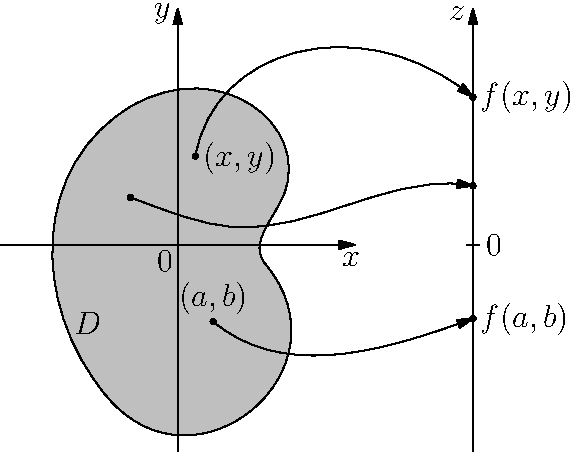
\includegraphics[width=\linewidth]{Images/Capitulo1/Funcion_dos_variables.pdf}
}

Una función de dos variables es una función cuyo dominio es un subconjunto de $\mathbb{R}^2$ y cuyo rango es un subconjunto de $\mathbb{R}$. Una manera de representar tal función es mediante un diagrama de flechas (véase la figura \ref{fig:Funcion_dos_variables}), donde el dominio $D$ se representa como un subconjunto del plano $x y$ y el rango es un conjunto de números sobre una recta real, que se muestra como un eje $z$. %Por ejemplo, si $f(x, y)$ representa la temperatura en un punto $(x, y)$ en una placa metálica plana con la forma de $D$, podemos considerar al eje $z$ como un termómetro que va mostrando el registro de temperaturas.

Si una función $f$ está dada por una fórmula y no se especifica dominio alguno, entonces se entiende que el dominio de $f$ será el conjunto de parejas $(x, y)$ para el cual la expresión dada es un número bien definido.

\begin{example}
    Para las siguientes funciones, evalúe $f(3, 2)$ y determine y grafique el dominio.
    \begin{tasks}(2)
        \task $\displaystyle f(x, y) = \frac{\sqrt{x + y + 1}}{x - 1}$
        \task $f(x, y) = x \ln (y^2 - x)$
    \end{tasks}
    \solucion
    \begin{enumerate}[label=\alph*)]
        \item Tenemos que\sideFigure[\label{Fig:Dominio_1}Representación geométrica del dominio de $\displaystyle f(x, y) = \frac{\sqrt{x + y + 1}}{x - 1}$]{
        \begin{tikzpicture}
            \filldraw[gray,opacity=0.5] (1.5,-2.5) --(2.5,-2.5) -- (2.5,2.5) -- (-2.5,2.5) -- (-2.5,1.5) -- (1.5,-2.5) -- cycle;
            \draw[-latex] (-2.5,0) -- (2.5,0) node[below left] {$x$};
            \draw[-latex] (0,-2.5) -- (0,2.5) node[below left] {$y$};
            \draw (-2.5,1.5) -- (1.5,-2.5);
            \draw[latex-] (-2,1) -- (-1.5,2) node[above] {$x + y + 1 = 0$};
            \node[below left] at (0,0) {$0$};
            \node[below left] at (-0.9,0) {$-1$};
            \node[left] at (0,-1.1) {$-1$};
            \draw[dash pattern=on 3pt off 3pt] (1,-2) -- (1,2.5);
            \node[right] at (1.1,1.5) {$x = 1$};
        \end{tikzpicture}
        }
        $$f(3, 2) = \frac{\sqrt{3 + 2 + 1}}{3 - 1} = \frac{\sqrt{6}}{2}$$
        La expresión para $f$ tiene sentido si el denominador no es cero y la cantidad dentro del signo de raíz cuadrada es no negativa. Entonces, el dominio de $f$ es
        $$D = \left\{ (x, y) \in \RR[2] \mid x + y + 1 \geq 0, x \neq 1 \right\}.$$
        La desigualdad $x + y + 1 \geq 0$, o bien, $y \geq -x - 1$, describe los puntos que quedan en o por arriba de la recta $y = -x - 1$, mientras que $x \neq 1$ significa que los puntos sobre la recta $x = 1$ tienen que ser excluidos del dominio. Vea la figura \ref{Fig:Dominio_1}.
        \item Tenemos que\sideFigure[\label{Fig:Dominio_2}Representación geométrica del dominio de $f(x, y) = x \ln (y^2 - x)$]{
        \begin{tikzpicture}
            \filldraw[gray,opacity=0.5] (-2.5,-2.5) rectangle (2.49,2.5);
            \node[below left] at (0,0) {$0$};
            \filldraw[rotate=-90,white] (-2.5,2.5) parabola bend (0,0) (2.5,2.5);
            \draw[rotate=-90,dash pattern=on 3pt off 3pt] (-2.5,2.5) parabola bend (0,0) (2.5,2.5);
            \draw[latex-] (1,1.5) -- (1.5,0.75) node[below] {$x = y^2$};
            \draw[-latex] (-2.5,0) -- (2.5,0) node[below left] {$x$};
            \draw[-latex] (0,-2.5) -- (0,2.5) node[below left] {$y$};
        \end{tikzpicture}
        }
        $$f(3, 2) = 3 \ln (2^2 - 3) = 0.$$
        Puesto que $\ln(y^2 - x)$ se define solo cuando $y^2 - x > 0$, es decir, $x < y^2$, el dominio de $f$ es
        $$D = \left\{ (x, y) \in \RR[2] \mid x < y^2 \right\}.$$
        Este es el conjunto de puntos a la izquierda de la parábola $x = y^2$. Vea la figura \ref{Fig:Dominio_2}.
    \end{enumerate}
\end{example}

\begin{example}
    Determine y grafique el dominio de las siguientes funciones:
    \begin{tasks}(2)
        \task $f(x, y) = \sqrt{x^2 + y^2 - 1}$
        \task $f(x, y) = \ln (x^2 + y^2 - 1)$
    \end{tasks}
    \newpage
    \solucion \sideFigure[\label{Fig:Dominio_3}Representación geométrica del dominio de $f(x, y) = \sqrt{x^2 + y^2 - 1}$]{
    \begin{tikzpicture}
        \filldraw[gray,opacity=0.5] (-2.5,-2.5) rectangle (2.5,2.5);
        \filldraw[white] (0,0) circle (1.5cm);
        \draw (0,0) circle (1.5cm);
        \draw[-latex] (-2.5,0) -- (2.5,0) node[below left] {$x$};
        \draw[-latex] (0,-2.5) -- (0,2.5) node[below left] {$y$};
        \node[below left] at (0,0) {$0$};
        \draw[latex-] (0.6,1.4) -- (1.3,2) node[above] {$x^2 + y^2 = 1$};
    \end{tikzpicture}
    }
    \begin{enumerate}[label=\alph*)]
        \item Siguiendo la misma idea el ejemplo anterior, la expresión para $f$ tiene sentido si la cantidad dentro del signo de raíz cuadrada es no negativa. Así, el dominio de $f$ es
        $$D = \left\{ (x, y) \in \RR[2] \mid x^2 + y^2 - 1 \geq 0 \right\}.$$
        La desigualdad $x^2 + y^2 - 1 \geq 0$, o bien, $x^2 + y^2 \geq 1$, describe los puntos que quedan en o fuera de la circunferencia $x^2 + y^2 = 1$.
        \item Puesto que $\ln (x^2 + y^2 - 1)$ se define solo cuando $x^2 + y^2 - 1 > 0$, es decir, $x^2 + y^2 > 1$ el dominio de $f$ es\sideFigure[\label{Fig:Dominio_4}Representación geométrica del dominio de $f(x, y) = \ln (x^2 + y^2 - 1)$]{
        \begin{tikzpicture}
            \filldraw[gray,opacity=0.5] (-2.5,-2.5) rectangle (2.5,2.5);
            \filldraw[white] (0,0) circle (1.5cm);
            \draw[dash pattern=on 3pt off 3pt] (0,0) circle (1.5cm);
            \draw[-latex] (-2.5,0) -- (2.5,0) node[below left] {$x$};
            \draw[-latex] (0,-2.5) -- (0,2.5) node[below left] {$y$};
            \node[below left] at (0,0) {$0$};
            \draw[latex-] (0.6,1.4) -- (1.3,2) node[above] {$x^2 + y^2 = 1$};
        \end{tikzpicture}
        }
        $$D = \left\{ (x, y) \in \RR[2] \mid x^2 + y^2 > 1 \right\}.$$
        Este es el conjunto de puntos que están fuera de la circunferencia sin tomar los puntos que están en $x^2 + y^2 = 1$.
    \end{enumerate}
\end{example}

\begin{definition}
    Una función de tres variables, $f$, es una regla que asigna a cada terna ordenada $(x, y, z)$ en un dominio $D \subseteq \RR[3]$ un único número real denotado por $f(x, y, z)$.
\end{definition}

\begin{example}
    Graficar el dominio de la siguiente función:
    $$f(x, y, z) = \sqrt{x^2 + y^2 + z^2 - 4} + \ln \left( \frac{1}{\sqrt{x^2 + y^2 -1}} \right).$$
    \solucion Procediendo como ejemplos anteriores, notemos que se debe cumplir que
    $$x^2 + y^2 + z^2 - 4 \geq 0 \quad \text{ y } \quad x^2 + y^2 - 1 > 0.$$
    Analicemos la primer desigualdad, si tomamos la igualdad, obtenemos
    \begin{align*}
        x^2 + y^2 + z^2 - 4 & \geq 0 \\
        x^2 + y^2 + z^2 & \geq 4
    \end{align*}
    la cual es una esfera centrada en el origen y de radio igual a $2$. Luego, tomando la segunda desigualdad, se sigue que
    \begin{align*}
        x^2 + y^2 - 1 & > 0 \\
        x^2 + y^2 & > 1
    \end{align*}
    Si se toma la igualdad, esta será un cilindro de radio igual a $1$. Así, el dominio de la función $f$ es todo el exterior tanto del cilindro, como de la esfera. La función puede tomar puntos del “contorno” de la esfera, pero no puede tomar puntos del “contorno” del cilindro. Es difícil dibujar con exactitud el dominio de $f$, pero puede mirar la figura \ref{funcion3d}.\sideFigure[\label{funcion3d}]{
    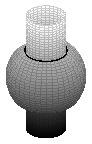
\includegraphics[width=\linewidth]{Images/Capitulo1/Dominio_de_funcion3d.pdf}
    }
\end{example}

\begin{example}
    Graficar el dominio de la siguiente función:
    $$f(x, y, z) = \sqrt{x^2 + y^2 - 4} + \frac{1}{y + z - 2}.$$
    \solucion Procediendo como ejemplos anteriores, notemos que se debe cumplir que
    $$x^2 + y^2 - 4 \geq 0 \quad \text{ y } \quad y + z - 2 \neq 0.$$
    Analicemos la primer desigualdad, si tomamos la igualdad, obtenemos\sideFigure[\label{dominiodefuncion3d}]{
    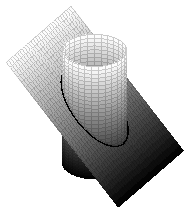
\includegraphics[width=\linewidth]{Images/Capitulo1/Dominio_de_funcion_en3D.pdf}
    }
    \begin{align*}
        x^2 + y^2 - 4 & \geq 0 \\
        x^2 + y^2 & \geq 4
    \end{align*}
    la cual es un cilindro centrado en el origen y de radio igual a $2$. Luego, analizando la segunda expresión; si tomamos la igualdad, se obtiene $y + z = 2$, el cual, es un plano. Por lo tanto, el dominio de $f$ es el conjunto de $(x, y, z)$ que quedan en o fuera del cilindro $x^2 + y^2 = 4$. Además, no puede tomar los puntos que conforma el plano $y + z - 2 = 0$, pues la división entre $0$ no está definida. Es difícil dibujar con exactitud el dominio de $f$, pero puede mirar la figura \ref{dominiodefuncion3d}.
\end{example}

\section{Gráficas de funciones y curvas de nivel}

\begin{reminder}
    Es importante destacar que el círculo es un caso particular de la elipse, pues recordemos que la expresión para una circunferencia centrada en el origen está dada por
    $$x^2 + y^2 = r^2$$
    donde $r$ es el radio de dicha circunferencia y es una constante real, mientras que una elipse está dada por
    $$\frac{x^2}{a^2} + \frac{y^2}{b^2} = 1$$
    siendo $a$ y $b$ constantes reales. Generalmente la elipse tiene dos ejes de diferentes longitudes y dos focos distintos, pero el círculo es una forma particular de elipse donde ambos ejes son idénticos y los dos focos coinciden en el centro del círculo. La elipse puede presentarse de dos maneras distintas: horizontalmente o verticalmente. Cuando decimos que una elipse está en posición horizontal, significa que su eje mayor se extiende más en el eje $x$, mientras que en la posición vertical, el eje mayor se extiende más en el eje $y$.
    \begin{figure}[h!]
        \centering
        \subfloat[Elipse horizontal: Cuando $a>b$]{
        \begin{tikzpicture}[scale=0.9]
            \draw[-latex] (-3,0) -- (3,0) node[below left] {$x$};
            \draw[-latex] (0,-3) -- (0,3) node[below left] {$y$};
            \draw (0,0) ellipse (2cm and 1cm);
        \end{tikzpicture}
        } \hfill
        \subfloat[Elipse vertical: Cuando $b>a$]{
        \begin{tikzpicture}[scale=0.9]
            \draw[-latex] (-3,0) -- (3,0) node[below left] {$x$};
            \draw[-latex] (0,-3) -- (0,3) node[below left] {$y$};
            \draw (0,0) ellipse (1cm and 2cm);
        \end{tikzpicture}
        }
        \caption{Representación de la elipse}
    \end{figure}
    
    \noindent La hipérbole es otra cónica, al igual que la elipse. Sin embargo, a diferencia de la elipse que tiene una forma cerrada, la hipérbole es una curva abierta que se extiende hacia el infinito en ambas direcciones. En términos algebraicos, la ecuación de una hipérbole con centro en el origen se expresa como:
    $$\frac{x^2}{a^2} - \frac{y^2}{b^2} = 1$$
    donde $a$ y $b$ son constantes reales. Al igual que la elipse, la hipérbole puede presentarse en dos configuraciones principales: horizontal y vertical. En el caso de una hipérbole horizontal, las ramas principales de la hipérbole se extienden horizontalmente a lo largo del eje $x$, mientras que en una hipérbole vertical, las ramas principales se extienden verticalmente a lo largo del eje $y$.
    \begin{figure}[h!]
        \centering
        \subfloat[Hipérbole horizontal: Cuando $a>b$]{
        \begin{tikzpicture}[scale=0.9]
            \draw[-latex] (-3,0) -- (3,0) node[below left] {$x$};
            \draw[-latex] (0,-3) -- (0,3) node[below left] {$y$};
            \draw[rotate=90,yshift=1cm] (-2,2) parabola bend (0,0) (2,2);
            \draw[rotate=-90,yshift=1cm] (-2,2) parabola bend (0,0) (2,2);
        \end{tikzpicture}
        } \hfill
        \subfloat[Hipérbole vertical: Cuando $b>a$]{
        \begin{tikzpicture}[scale=0.9]
            \draw[-latex] (-3,0) -- (3,0) node[below left] {$x$};
            \draw[-latex] (0,-3) -- (0,3) node[below left] {$y$};
            \draw[yshift=1cm] (-2,2) parabola bend (0,0) (2,2);
            \draw[rotate=180,yshift=1cm] (-2,2) parabola bend (0,0) (2,2);
        \end{tikzpicture}
        }
        \caption{Representación de la hipérbole}
    \end{figure}
\end{reminder}
%Otro modo de visualizar el comportamiento de una función de dos variables es considerar su gráfica

\sideFigure[\label{fig:1.6defuncion}]{\vspace{2cm}
\tdplotsetmaincoords{75}{110}
\begin{tikzpicture}[tdplot_main_coords,scale=2]
    \draw[thick,-latex] (0,0,0) coordinate(O) -- (2.5,0,0) node[anchor=north east] (x) {$x$};
    \draw[thick,-latex] (0,0,0) -- (0,1.5,0) node[anchor=north west] (y) {$y$};
    \draw[thick,-latex] (0,0,0) -- (0,0,2.5) node[anchor=south] (z) {$z$};
    \begin{scope}[xshift=0mm,rotate=-10]
        \tikzfading[name=fade right,
            left color=transparent!00,
            right color=transparent!60] ;
            \filldraw[black!30,path fading=fade right,fill opacity=0.5,
            ]  plot[variable=\x,samples=180,domain=-90:270] ({1.2*cos(\x)},{sin(\x)},{0});
            \draw plot[variable=\x,samples=180,domain=-90:270] ({1.2*cos(\x)},{sin(\x)},{0});
    \end{scope}
    \coordinate[label={[name=Plabel,xshift=0.5cm,yshift=1.7cm]above right:{$\big(x, y, f(x, y)\big)$}}] (P) at (0.2,0.5,1.2);
    \draw[-latex,shorten >=2.5pt] (Plabel) --(P);
    \fill (P) circle (1pt);
    \coordinate[label=below:{$(x, y, 0)$}] (Q) at (0.2,0.5,0);
    \fill (Q) circle (1pt);
    \draw[thick,] (P) -- (Q);
    \draw[thick,decoration={brace,raise=2.5pt},decorate] (P) -- (Q) node[midway,right=2mm]{$f(x, y)$};
    \draw[fill=gray,fill opacity=0.5,name path=back,->] plot[variable=\x,samples=180,domain=50:270] ({1.2*cos(\x)},{sin(\x)},{1.2+0.4*cos(2*\x)}) to[out=30,in=160] cycle;
    \draw[fill=gray,fill opacity=0.5,name path=front] plot[variable=\x,samples=180,domain=-90:50] ({1.2*cos(\x)},{sin(\x)},{1.2+0.4*cos(2*\x)}) to[out=160,in=30] cycle;
    \node[xshift=-0.2cm,yshift=1cm] at (0.2,0.5,1.2) {$S$};
    \node[xshift=-1.5cm,yshift=0.2cm] at (0.2,0.5,0) {$D$};
\end{tikzpicture}
}

\sideFigure[Un ejemplo común de las curvas de nivel son los mapas topográficos de regiones montañosas]{
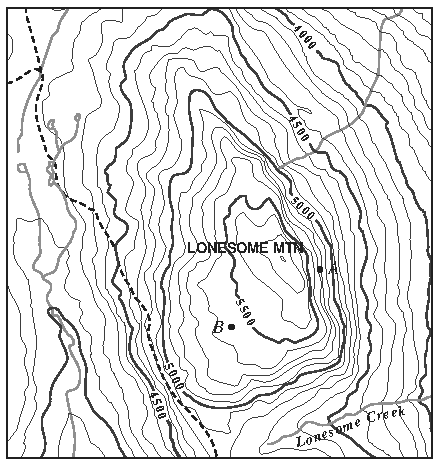
\includegraphics[width=\linewidth]{Images/Capitulo1/Cartografico.pdf}
}
\sideFigure[\label{fig:curvasdenivelre}Representación geométrica de las curvas de nivel de una función]{
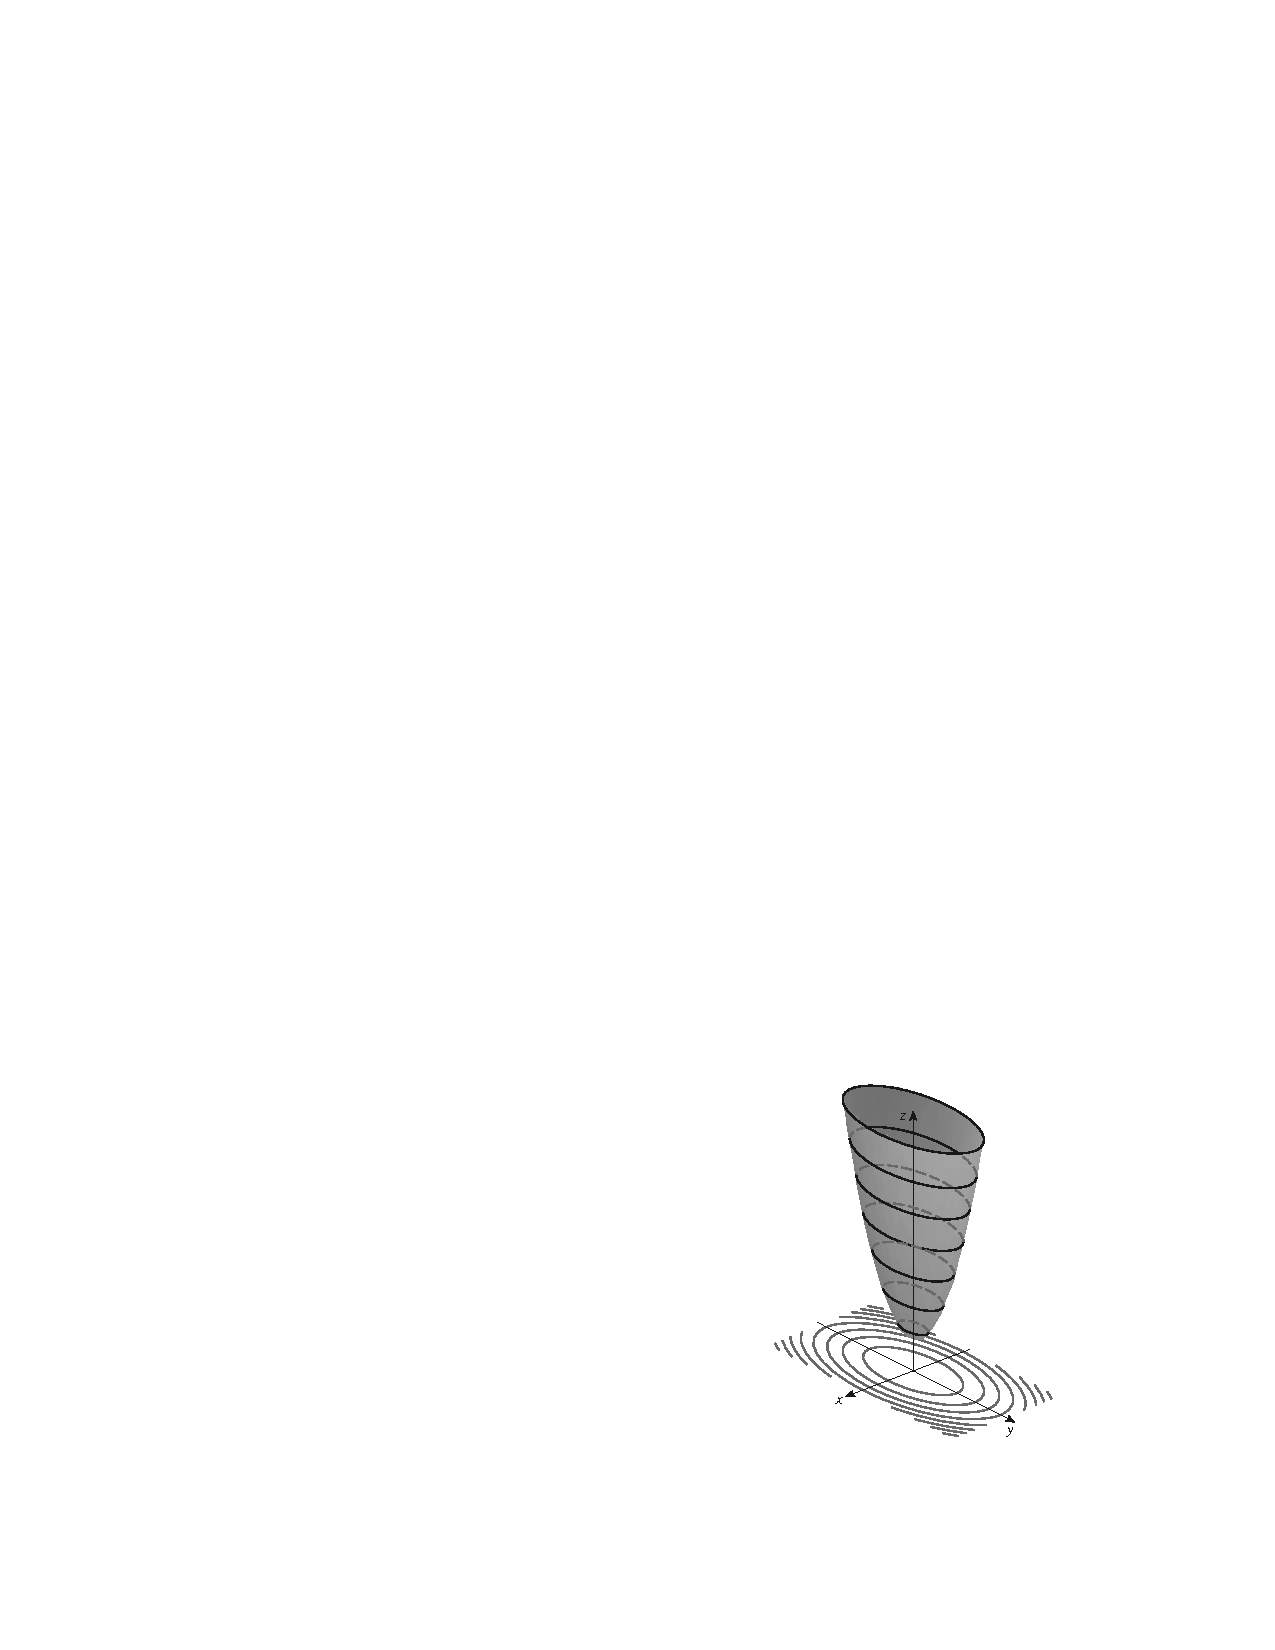
\includegraphics[width=\linewidth]{Images/Capitulo1/Curvas_de_nivelBW.pdf}
}
\vspace{-0.5cm}
\begin{definition}
    Sea $f:D \subseteq \RR[n] \longrightarrow \RR$ una función, entonces la gráfica de $f$ es
    $$\mathcal{G}(f) = \left\{ \big(x, f(x)\big) \mid x \in D \right\} \subseteq \RR[n+1].$$
\end{definition}

\begin{observation}
    Si $f$ es una función de dos variables con dominio $D$, entonces la gráfica de $f$ es el conjunto de todos los puntos $(x, y, z)$ en $\RR[3]$ tal que $(x, y)$ y $z = f(x, y)$ está en $D$.
\end{observation}

Así como la gráfica de una función $f$ de una variable es una curva $C$ con ecuación $y = f (x)$, la gráfica de una función $f$ de dos variables es una superficie $S$ cuya ecuación es $z = f (x, y)$. Podemos visualizar la gráfica $S$ de $f$ directamente sobre o abajo de su dominio $D$ en el plano $xy$ (véase la figura \ref{fig:1.6defuncion}).

Un método para poder graficar funciones de dos funciones es mediante un mapa de curvas de nivel en el cual puntos de elevación igual se unen para formar líneas de contorno o curvas de nivel. Las curvas de nivel son líneas imaginarias que se utilizan para representar superficies tridimensionales en dos dimensiones, como mapas topográficos o gráficos de funciones de dos variables. Estas curvas conectan puntos que tienen la misma altura o el mismo valor de la función en el caso de las superficies. Por ejemplo, en un mapa topográfico, las curvas de nivel unen puntos que tienen la misma elevación sobre el nivel del mar. Al observar estas curvas, podemos entender la variación de la elevación o la función en diferentes áreas de la superficie, lo que proporciona una representación visual y comprensible del terreno o de la función en cuestión. %Las curvas de nivel son una herramienta poderosa en diversas áreas, desde la cartografía hasta la ingeniería y las ciencias ambientales, facilitando la interpretación y el análisis de datos espaciales y funcionales.

\begin{definition}
    Se define la \textbf{curva de nivel} de $f$ correspondiente al valor $k \in \RR$ como
    $$\mathcal{C}_k(f) = \left\{ (x_1, x_2, \dots, x_n) \in D \mid f(x_1, x_2, \dots, x_n) = k \right\}.$$
\end{definition}

\begin{observation}
    Una curva de nivel $f(x, y) = k$ es el conjunto de todos los puntos en el dominio de $f$ en el cual $f$ toma un valor dado $k$. En otras palabras, señala dónde tiene una altura $k$ la gráfica de $f$. Vea la imagen \ref{fig:curvasdenivelre}.
\end{observation}

\begin{example}
    Graficar la función $f(x, y) = x^{2} - y^{2}$.\\
    \solucion Para graficar la función $f$, obtengamos algunas curvas de nivel. Sea $z = x^2 - y^2$,
    \begin{itemize}
        \item Si $z = 0$, entonces
        \begin{align*}
            0 & = x^2 - y^2 \\
            & = (x-y)(x+y);
        \end{align*}
        así que $y = x$ o $y = -x$. Es decir, obtenemos dos rectas perpendiculares.
        \item Si $z = 1$, entonces
        $$1 = x^2 - y^2;$$
        así que obtenemos una hipérbole (cuando $y = 0$, $x = \pm 1$).
        \item Si $z = 2$, entonces
        $$2 = x^2 - y^2;$$
        así que obtenemos una hipérbole (cuando $y = 0$, $x = \pm \sqrt{2}$).
        \item Si $z = 3$, entonces
        $$3 = x^2 - y^2;$$
        así que obtenemos una hipérbole (cuando $y = 0$, $x = \pm \sqrt{3}$).
    \end{itemize}
    Entonces, las curvas de nivel (en el plano $xy$) son como se muestran a continuación:
    \begin{figure}[h!]
        \centering
        \subfloat[Cuando $z = 0$]{
        \begin{tikzpicture}
            \draw[-latex] (-2.5,0) -- (2.5,0) node[below left] {$x$};
            \draw[-latex] (0,-2.5) -- (0,2.5) node[below left] {$y$};
            \draw (-2.5,-2.5) -- (2.5,2.5);
            \draw (-2.5,2.5) -- (2.5,-2.5);
        \end{tikzpicture}
        } \hfill
        \subfloat[Cuando $z = 1$]{
        \begin{tikzpicture}
            \draw[-latex] (-2.5,0) -- (2.5,0) node[below left] {$x$};
            \draw[-latex] (0,-2.5) -- (0,2.5) node[below left] {$y$};
            \draw[rotate=90,yshift=0.5cm] (-2,2) parabola bend (0,0) (2,2);
            \draw[rotate=-90,yshift=0.5cm] (-2,2) parabola bend (0,0) (2,2);
            \node[below] at (-1,0) {$-1$};
            \node[below] at (1,0) {$1$};
        \end{tikzpicture}
        } \\
        \subfloat[Cuando $z = 2$]{
        \begin{tikzpicture}
            \draw[-latex] (-2.5,0) -- (2.5,0) node[below left] {$x$};
            \draw[-latex] (0,-2.5) -- (0,2.5) node[below left] {$y$};
            \draw[rotate=90,yshift=0.7cm] (-2,1.8) parabola bend (0,0) (2,1.8);
            \draw[rotate=-90,yshift=0.7cm] (-2,1.8) parabola bend (0,0) (2,1.8);
            \node[below] at (-1.2,0) {$-\sqrt{2}$};
            \node[below] at (1.2,0) {$\sqrt{2}$};
        \end{tikzpicture}
        } \hfill
        \subfloat[Cuando $z = 3$]{
        \begin{tikzpicture}
            \draw[-latex] (-2.5,0) -- (2.5,0) node[below left] {$x$};
            \draw[-latex] (0,-2.5) -- (0,2.5) node[below left] {$y$};
            \draw[rotate=90,yshift=0.86cm] (-2,1.6) parabola bend (0,0) (2,1.6);
            \draw[rotate=-90,yshift=0.86cm] (-2,1.6) parabola bend (0,0) (2,1.6);
            \node[below] at (-1.4,0) {$-\sqrt{3}$};
            \node[below] at (1.4,0) {$\sqrt{3}$};
        \end{tikzpicture}
        }
        \caption{Algunas curvas de nivel de $x^2 - y^2$}
    \end{figure}
    \newpage
    \noindent Por último, encontremos los “perfiles” de la función. Si $y = 0$, entonces $z = x^2$; y si $x = 0$, entonces $z = -x^2$. Por tanto, la gráfica de la función $f(x, y) = x^{2} - y^{2}$ está dada como sigue:
    \begin{figure}[h!]
        \centering
        \begin{tikzpicture}
            \begin{axis}[view={-20}{45},
                %axis lines=center,
                %axis on top,
                colormap/blackwhite
                ]
                \addplot3 [surf,
                draw=black,
                domain=-9:9,
                domain y=-9:9,
                ] {x^2-y^2};
            \end{axis}
        \end{tikzpicture}
        \caption{Gráfica de la función $x^2 - y^2$}
    \end{figure}
\end{example}

\section{Definición y ejemplos de normas}

Una norma en el contexto del cálculo de varias variables es una función que asigna a cada vector en un espacio vectorial una magnitud no negativa, de modo que satisface ciertas propiedades fundamentales. La norma más comúnmente utilizada es la norma euclidiana o norma $\ell_2$, que se define como la raíz cuadrada de la suma de los cuadrados de las componentes del vector. Esta norma captura la noción geométrica de distancia y es fundamental en el análisis vectorial y el cálculo diferencial e integral.

Además de la norma euclidiana, existen otras normas importantes en el cálculo de varias variables, como la norma $\ell_1$ (que es la suma de los valores absolutos de las componentes del vector), la norma $\ell_{\infty}$ (que es el máximo valor absoluto de las componentes del vector), entre otras.

\begin{definition}
    Sea $V$ un espacio vectorial sobre $K$ (donde $K$ generalmente es el conjunto de los números reales $\mathbb{R}$ o los números complejos $\mathbb{C}$). La norma en $V$ es una función $\| \quad \| : V \longrightarrow \RR$ que satisface las siguientes propiedades: Para todo $\mathbf{x}$, $\mathbf{y} \in V$ y $\lambda \in K$
    \begin{enumerate}[label=\roman*.]
        \item $\| \mathbf{x} \| \geq 0$,
        \item $\| \mathbf{x} \| = 0$ si y solo si $\mathbf{x} = \mathbf{0}$,
        \item $\| \lambda \mathbf{x} \| = |\lambda| \| \mathbf{x} \|$,
        \item $\| \mathbf{x} + \mathbf{y} \| \leq \| \mathbf{x} \| + \| \mathbf{y} \|$ (desigualdad del triángulo).
    \end{enumerate}
\end{definition}

\begin{example}
    En $\RR$, sea $\| \mathbf{x} \| = |x|$, probemos entonces que $\| \quad \|$ cumple las cuatro propiedades establecidas en la definición previa.
    \begin{enumerate}[label=\roman*.]
        \item Sea $\mathbf{x} \in \RR$, entonces
        \begin{align*}
            \| \mathbf{x} \| & = |x| \\
            & \geq 0 
        \end{align*}
        Por tanto, $\| \mathbf{x} \| \geq 0$.
        \item Por el curso de Cálculo I,
        $$\| \mathbf{x} \| = 0_{\RR} \Longleftrightarrow |x| = 0_{\RR} = 0 \Longleftrightarrow x = 0 = \mathbf{0}_V.$$
        Por tanto, $\| \mathbf{x} \| = 0$ si y solo si $\mathbf{x} = \mathbf{0}$.
        \item Sea $\mathbf{x} \in \RR$ y $\lambda \in \RR$, entonces
        \begin{align*}
            \| \lambda \mathbf{x} \| & = |\lambda x| \\
            & = |\lambda| |x| \\
            & = |\lambda| \| \mathbf{x} \| 
        \end{align*}
        Por tanto, $\| \lambda \mathbf{x} \| = |\lambda| \| \mathbf{x} \|$.
        \item Sean $\mathbf{x}$, $\mathbf{y} \in \RR$, entonces
        \begin{align*}
            \| \mathbf{x} + \mathbf{y} \| & = |x + y| \\
            & \leq |x| + |y| \\
            & = \| \mathbf{x} \| + \| \mathbf{y} \|
        \end{align*}
        Por tanto, $\| \mathbf{x} + \mathbf{y} \| \leq \| \mathbf{x} \| + \| \mathbf{y} \|$.
    \end{enumerate}
    Dado que $\| \quad \|$ satisface las cuatro propiedades de una norma, concluimos que  $\| \quad \|$ es una norma.
\end{example}

\begin{observation}
    En el ejemplo anterior, aunque el espacio vectorial era $\RR$, es importante distinguir entre los vectores y los números reales, pues son cosas muy distintas. Por tanto, los vectores los representaremos utilizando letras en negrita para distinguirlos de los números reales.
\end{observation}

\begin{definition}
    En $\RR[2]$, sea $\| (x, y) \|_1 = |x| + |y|$, probemos entonces que $\| \quad \|_1$ cumple las cuatro propiedades establecidas en la definición previa.
    \begin{enumerate}[label=\roman*.]
        \item Sea $(x, y) \in \RR[2]$, entonces
        \begin{align*}
            \| (x, y) \|_1 & = \smallunderbrace{|x|}_{\geq 0} + \smallunderbrace{|y|}_{\geq 0} \\
            & \geq 0
        \end{align*}
        Así, $\| (x, y) \|_1 \geq 0$.
        \item \begin{enumerate}
            \item[$\Rightarrow)$] Sea $(x, y) \in \RR[2]$, entonces
            $$\| (x, y) \|_1 = |x| + |y|,$$
            así que $|x| = 0$ y $|y| = 0$. Es decir, $x = 0$ y $y = 0$. Así pues, se sigue que $(x, y) = (0, 0) = \mathbf{0}$.
            \item[$\Leftarrow)$] Sea $\mathbf{0} \in \RR[2]$ con $\mathbf{0} = (0, 0)$, entonces
            \begin{align*}
                \| (0, 0) \|_1 & = |0| + |0| \\
                & = 0 + 0 \\
                & = 0
            \end{align*}
            Por lo tanto, $\| (0, 0) \|_1 = 0$.
        \end{enumerate}
        \item Sea $(x, y) \in \RR[2]$ y $\lambda \in \RR$, entonces
        \begin{align*}
            \| \lambda (x, y) \|_1 & = \| (\lambda x, \lambda y) \|_1 \\
            & = |\lambda x| + |\lambda y| \\
            & = |\lambda| |x| + |\lambda| |y| \\
            & = \lambda \left( |x| + |y| \right) \\
            & = |\lambda| \| (x, y) \|_1
        \end{align*}
        Por tanto, $\| \lambda (x, y) \|_1 = |\lambda| \| (x, y) \|_1$.
        \item Sean $(x, y)$, $(u, v) \in \RR[2]$, entonces
        \begin{align*}
            \| (x, y) + (u, v) \|_1 & = \| (x + u, y + v) \|_1 \\
            & = |x + u| + |y + v| \\
            & \leq |x| + |u| + |y| + |v| \\
            & = |x| + |y| + |u| + |v| \\
            & = \| (x, y) \|_1 + \| (u, v) \|_1
        \end{align*}
        Por tanto, $\| (x, y) + (u, v) \|_1 \leq \| (x, y) \|_1 + \| (u, v) \|_1$.
    \end{enumerate}
    Dado que $\| \quad \|_1$ satisface las cuatro propiedades de una norma, concluimos que  $\| \quad \|_1$ es una norma.
\end{definition}

\begin{example}
    En $\RR[2]$, sea $\| (x, y) \|_{\infty} = \max \left\{ |x|, |y| \right\}$, probemos entonces que $\| \quad \|_{\infty}$ cumple las cuatro propiedades establecidas en la definición previa.
    \begin{enumerate}[label=\roman*.]
        \item Sea $(x, y) \in \RR[2]$, entonces
        $$\| (x, y) \|_{\infty} = \max \left\{ |x|, |y| \right\}.$$
        Notemos que si $\max \left\{ |x|, |y| \right\} = |x|$, entonces $\| (x, y) \|_{\infty} = |x| \geq 0$. De manera análoga, si $\max \left\{ |x|, |y| \right\} = |y|$, entonces $\| (x, y) \|_{\infty} = |y| \geq 0$. Así que, en cualquiera de los dos casos, $\| (x, y) \|_{\infty} \geq 0$.
        \item \begin{enumerate}
            \item[$\Rightarrow)$] Sea $(x, y) \in \RR[2]$, entonces
            $$\| (x, y) \|_{\infty} = \max \left\{ |x|, |y| \right\}.$$
            Si $\max \left\{ |x|, |y| \right\} = |x|$, entonces implica que $|y| \leq |x| = 0$. Sin embargo, $0 \leq |y| \leq |x| = 0$, lo que conduce a $|x| = 0$ y $|y| = 0$. Por lo tanto, $x = 0$ y $y = 0$, es decir, $(x, y) = (0, 0) = \mathbf{0}$.
            \item[$\Leftarrow)$] Si $(x, y) = \mathbf{0}$, entonces $x = 0$ y $y = 0$. Así,
            \begin{align*}
                \| (x, y) \|_{\infty} & = \| (0, 0) \|_{\infty} \\
                & = \max \left\{ |0|, |0| \right\} \\
                & = \max \left\{ 0 \right\} \\
                & = 0
            \end{align*}
            Por lo tanto, $\| (0, 0) \|_{\infty} = 0$.
        \end{enumerate}
    \end{enumerate}
    \begin{adjustwidth}{0mm}{-\wholeMargin}
        \noindent\begin{minipage}[c]{8.2cm}
            \begin{enumerate}[label=\roman*.,start=3]
                \item Sea $(x, y) \in \RR[2]$ y $\lambda \in \RR$, entonces
                \begin{align*}
                    \| \lambda (x, y) \|_{\infty} & = \| (\lambda x, \lambda y) \|_{\infty} \\
                    & = \max \left\{ |\lambda x|, |\lambda y| \right\} \\
                    & = |\lambda| \max \left\{ |x|, |y| \right\} \\
                    & = |\lambda| \| (x, y) \|_{\infty}
                \end{align*}
                Por tanto $\| \lambda (x, y) \|_{\infty} = |\lambda| \| (x, y) \|_{\infty}$.
            \end{enumerate}
        \end{minipage}\hfill
        \begin{minipage}[c]{9.5cm}
            \colorbox{gray!20}{\parbox[c]{\dimexpr\linewidth-3pt-2\fboxsep-2\fboxrule}{\footnotesize
            Por el curso de Cálculo I, se establece que
            $$\max \left\{ |\lambda| |x|, |\lambda| |y| \right\} = |\lambda| \max \left\{ |x|, |y| \right\}.$$
            En efecto: Si $\lambda = 0$, es evidente que la anterior igualdad se cumple. En caso contrario, es decir, $\lambda \neq 0$, procedemos por casos:\\[-2mm]
            \begin{enumerate}[label=\roman*)]
                \item Si $|\lambda| |x| \leq |\lambda| |y|$, entonces $\max \left\{ |\lambda| |x|, |\lambda| |y| \right\} = |\lambda| |y|$ y $|x| \leq |y|$, pues $\lambda \neq 0$ y además, $|\lambda| > 0$. Por lo tanto $|\lambda| \max \left\{ |x|, |y| \right\} = |\lambda| |y|$. Así, se verifica la igualdad.
                \item Se procede de manera análoga a (i).
            \end{enumerate}
        }}
        \end{minipage}
    \end{adjustwidth}\newpage
    \begin{enumerate}[label=\roman*.,start=4]
        \item Sean $(x, y)$, $(u, v) \in \RR[2]$, entonces
        \begin{align*}
            \| (x, y) + (u, v) \|_{\infty} & = \| (x + u, y + v) \|_{\infty} \\
            & = \max \left\{ |x + u|, |y + v| \right\} \\
            & \leq \max \left\{ |x| + |u|, |y| + |v| \right\} \\
            & \leq \max \left\{ |x|, |y| \right\} + \max \left\{ |u|, |v| \right\} \\
            & = \| (x, y) \|_{\infty} + \| (u, v) \|_{\infty}
        \end{align*}
    \end{enumerate}
    Dado que $\| \quad \|_{\infty}$ satisface las cuatro propiedades de una norma, concluimos que $\| \quad \|_{\infty}$ es una norma.
\end{example}

\begin{theorem}[Desigualdad de Cauchy-Schwarz]
    Sea $V$ un $k$-espacio vectorial con producto interno $\langle \, , \rangle$. Sean $\mathbf{x}$, $\mathbf{y} \in V$, entonces se cumple
    $$| \langle \mathbf{x}, \mathbf{y} \rangle | \leq \| \mathbf{x} \| \| \mathbf{y} \|.$$
    \demostracion Sean $\mathbf{x}$, $\mathbf{y} \in V$, con $\mathbf{y} \neq \mathbf{0}$ y sea $\lambda \in K$. Consideremos al vector $\mathbf{x} + \lambda \mathbf{y}$, entonces se tiene \vspace{-0.7cm}
    \begin{adjustwidth}{0mm}{-\wholeMargin}
        \noindent\begin{minipage}[c]{10cm}
            \begin{align*}
                0 \leq \| \mathbf{x} + \lambda \mathbf{y} \|^2 & = \langle \mathbf{x} + \lambda\mathbf{y}, \mathbf{x} + \lambda\mathbf{y} \rangle \\
                & = \langle \mathbf{x}, \mathbf{x} + \lambda \mathbf{y} \rangle + \langle \lambda \mathbf{y}, \mathbf{x} + \lambda\mathbf{y} \rangle \\
                & = \langle \mathbf{x}, \mathbf{x} \rangle + \langle \mathbf{x}, \lambda \mathbf{y} \rangle + \langle \lambda \mathbf{y}, \mathbf{x} \rangle + \langle \lambda \mathbf{y}, \lambda \mathbf{y} \rangle \\
                & = \langle \mathbf{x}, \mathbf{x} \rangle + \overline{\lambda} \langle \mathbf{x}, \mathbf{y} \rangle + \lambda \langle \mathbf{y}, \mathbf{x} \rangle + \lambda \langle \mathbf{y}, \lambda \mathbf{y} \rangle \\
                & = \langle \mathbf{x}, \mathbf{x} \rangle + \overline{\lambda} \langle \mathbf{x}, \mathbf{y} \rangle + \lambda \overline{\langle \mathbf{x}, \mathbf{y} \rangle} + \lambda\overline{\lambda} \langle \mathbf{y}, \mathbf{y} \rangle \\
                & = \| \mathbf{x} \|^2 + \overline{\lambda} \langle \mathbf{x}, \mathbf{y} \rangle + \lambda \overline{\langle \mathbf{x}, \mathbf{y} \rangle} + |\lambda|^2 \| \mathbf{y} \|^2
            \end{align*}
        \end{minipage}\hfill
        \begin{minipage}[c]{7.7cm}
            \colorbox{gray!20}{\parbox[c]{\dimexpr\linewidth-3pt-2\fboxsep-2\fboxrule}{\footnotesize
            \textbf{Recordatorio:} Sea $V$ un $k$-espacio vectorial. Un producto interno en $V$ es una función $\langle \, , \rangle :V \times V \longrightarrow K$ tal que\\[-2mm]
            \begin{enumerate}[label=\roman*)]
                \item $\langle \mathbf{x} + \mathbf{y}, \mathbf{z} \rangle = \langle \mathbf{x}, \mathbf{z} \rangle + \langle \mathbf{y}, \mathbf{z} \rangle$, $\forall \mathbf{x}$, $\mathbf{y}$, $\mathbf{z} \in V$.
                \item $\langle \lambda \mathbf{x}, \mathbf{y} \rangle = \lambda \langle \mathbf{x}, \mathbf{y} \rangle$, $\forall \lambda \in K$ y $\forall \mathbf{x}$, $\mathbf{y} \in V$.
                \item $\langle \mathbf{x}, \mathbf{y} \rangle = \overline{\langle \mathbf{y}, \mathbf{x} \rangle}$, $\forall \mathbf{x}$, $\mathbf{y} \in V$.
                \item Si $\mathbf{x} \in V$, $\mathbf{x} \neq \mathbf{0}$, entonces $\langle \mathbf{x}, \mathbf{x} \rangle > 0$.\\[-2mm]
            \end{enumerate}
            Además, el producto interno es homogéneo conjugado respecto al segundo argumento, es decir,
            $$\langle \mathbf{x}, \lambda \mathbf{y} \rangle = \overline{\lambda} \langle \mathbf{x}, \mathbf{y} \rangle , \forall \lambda \in K.$$
        }}
        \end{minipage}
    \end{adjustwidth}\vspace{-0.3cm}
    Así,
    $$0 \leq \| \mathbf{x} + \lambda \mathbf{y} \|^2 = \| \mathbf{x} \|^2 + \overline{\lambda} \langle \mathbf{x}, \mathbf{y} \rangle + \lambda \overline{\langle \mathbf{x}, \mathbf{y} \rangle} + |\lambda|^2 \| \mathbf{y} \|^2.$$
    Entonces
    \begin{equation}
        0 \leq \| \mathbf{x} \|^2 + \overline{\lambda} \langle \mathbf{x}, \mathbf{y} \rangle + \lambda \overline{\langle \mathbf{x}, \mathbf{y} \rangle} + |\lambda|^2 \| \mathbf{y} \|^2, \label{desigualdad-cauchy}
    \end{equation}
    lo cual se cumple para toda $\lambda \in K$, en particular para $\displaystyle \lambda = \frac{(-1)\langle \mathbf{x}, \mathbf{y} \rangle}{\| \mathbf{y} \|^2}$. Además, es evidente que $\displaystyle \overline{\lambda} = \frac{(-1)\overline{\langle \mathbf{x}, \mathbf{y} \rangle}}{\| \mathbf{y} \|^2}$. Así que,
    $$|\lambda|^2 = \frac{(-1)\langle \mathbf{x}, \mathbf{y} \rangle}{\| \mathbf{y} \|^2} \cdot \frac{(-1)\overline{\langle \mathbf{x}, \mathbf{y} \rangle}}{\| \mathbf{y} \|^2} = \frac{|\langle \mathbf{x}, \mathbf{y} \rangle|^2}{\| \mathbf{y} \|^4}.$$
    Sustituyendo $\lambda$, $\overline{\lambda}$ y $|\lambda|^2$ en la expresión \eqref{desigualdad-cauchy}, se sigue que
    \begin{align*}
        0 & \leq \| \mathbf{x} \|^2 - \frac{\overline{\langle \mathbf{x}, \mathbf{y} \rangle}}{\| \mathbf{y} \|^2} \langle \mathbf{x}, \mathbf{y} \rangle - \frac{\langle \mathbf{x}, \mathbf{y} \rangle}{\| \mathbf{y} \|^2} \overline{\langle \mathbf{x}, \mathbf{y} \rangle} + \frac{|\langle \mathbf{x}, \mathbf{y} \rangle|^2}{\| \mathbf{y} \|^4} \| \mathbf{y} \|^2 \\
        & = \| \mathbf{x} \|^2 - \frac{|\langle \mathbf{x}, \mathbf{y} \rangle|^2}{\| \mathbf{y} \|^2} - \frac{|\langle \mathbf{x}, \mathbf{y} \rangle|^2}{\| \mathbf{y} \|^2} + \frac{|\langle \mathbf{x}, \mathbf{y} \rangle|^2}{\| \mathbf{y} \|^2} \\
        & = \| \mathbf{x} \|^2 - \frac{|\langle \mathbf{x}, \mathbf{y} \rangle|^2}{\| \mathbf{y} \|^2}
    \end{align*}
    Entonces
    $$\frac{|\langle \mathbf{x}, \mathbf{y} \rangle|^2}{\| \mathbf{y} \|^2} \leq \| \mathbf{x} \|^2,$$
    de donde se sigue que
    $$|\langle \mathbf{x}, \mathbf{y} \rangle|^2 \leq \| \mathbf{x} \|^2 \| \mathbf{y} \|^2.$$\newpage\noindent
    Así, finalmente obtenemos que
    $$|\langle \mathbf{x}, \mathbf{y} \rangle| \leq \| \mathbf{x} \| \| \mathbf{y} \|.$$
\end{theorem}

\begin{observation}
    Si $\mathbf{x}$ e $\mathbf{y}$ son linealmente dependientes, entonces
    $$|\langle \mathbf{x}, \mathbf{y} \rangle| = \| \mathbf{x} \| \| \mathbf{y} \|.$$
    Si $\mathbf{x}$ e $\mathbf{y}$ son linealmente independientes, entonces
    $$|\langle \mathbf{x}, \mathbf{y} \rangle| \leq \| \mathbf{x} \| \| \mathbf{y} \|.$$
\end{observation}

\begin{example}
    Sea $V$ un $k$-espacio vectorial con producto interno $\langle \, , \rangle$. Sean $\mathbf{x}$, $\mathbf{y} \in V$, entonces
    $$\| \mathbf{x} \| = \sqrt{\langle \mathbf{x}, \mathbf{x} \rangle}$$
    es una norma. \\
    \demostracion Probemos que $\| \mathbf{x} \|$ cumple las cuatro propiedades de una norma.
    \begin{enumerate}[label=\roman*.]
        \item Sea $\mathbf{x} \in V$,
        $$\| \mathbf{x} \| = \sqrt{\langle \mathbf{x}, \mathbf{x} \rangle} \geq 0.$$
        Por lo tanto $\| \mathbf{x} \| \geq 0$.
        \item Por las propiedades del producto interno, se sigue que
        $$0 = \| \mathbf{x} \| \Longleftrightarrow \sqrt{\langle \mathbf{x}, \mathbf{x} \rangle} \Longleftrightarrow \langle \mathbf{x}, \mathbf{x} \rangle \Longleftrightarrow \mathbf{x} = \mathbf{0}.$$
        Por tanto, $\| \mathbf{x} \| = 0$ si y solo si $\mathbf{x} = \mathbf{0}$.
        \item Sean $\mathbf{x} \in V$ y $\lambda \in K$,
        \begin{align*}
            \| \lambda \mathbf{x} \| & = \sqrt{\langle \lambda \mathbf{x}, \lambda \mathbf{x} \rangle} \\
            & = \sqrt{\lambda \langle \mathbf{x}, \lambda \mathbf{x} \rangle} \\
            & = \sqrt{\lambda \overline{\lambda} \langle \mathbf{x}, \mathbf{x} \rangle} \\
            & = \sqrt{\lambda \overline{\lambda}} \sqrt{\langle \mathbf{x}, \mathbf{x} \rangle} \\
            & = |\lambda| \| \mathbf{x} \|
        \end{align*}
        Por tanto, $\| \lambda \mathbf{x} \| = |\lambda| \| \mathbf{x} \|$.
        \item Sean $\mathbf{x}$, $\mathbf{y} \in V$, entonces
        \begin{align*}
            \| \mathbf{x} + \mathbf{y} \|^2 & = \langle \mathbf{x} + \mathbf{y}, \mathbf{x} + \mathbf{y} \rangle \\
            & = \langle \mathbf{x}, \mathbf{x} + \mathbf{y} \rangle + \langle \mathbf{y}, \mathbf{x} + \mathbf{y} \rangle \\
            & = \langle \mathbf{x}, \mathbf{x} \rangle + \langle \mathbf{x}, \mathbf{y} \rangle + \langle \mathbf{y}, \mathbf{x} \rangle + \langle \mathbf{y}, \mathbf{y} \rangle \\
            & = \| \mathbf{x} \|^2 + \langle \mathbf{x}, \mathbf{y} \rangle + \overline{\langle \mathbf{x}, \mathbf{y} \rangle} + \| \mathbf{y} \|^2 \\
            & = \| \mathbf{x} \|^2 + 2 \operatorname{Re} \left( \langle \mathbf{x}, \mathbf{y} \rangle \right) + \| \mathbf{y} \|^2 \\
            & \leq \| \mathbf{x} \|^2 + 2 \left| \langle \mathbf{x}, \mathbf{y} \rangle \right| + \| \mathbf{y} \|^2 \\
            & \leq \| \mathbf{x} \|^2 + 2 \| \mathbf{x} \| \| \mathbf{y} \| + \| \mathbf{y} \|^2 \\
            & = \left( \| \mathbf{x} \| + \| \mathbf{y} \| \right)^2
        \end{align*}
        Entonces
        $$\| \mathbf{x} + \mathbf{y} \|^2 \leq \left( \| \mathbf{x} \| + \| \mathbf{y} \| \right)^2,$$
        por lo que
        $$\| \mathbf{x} + \mathbf{y} \| \leq \| \mathbf{x} \| + \| \mathbf{y} \|.$$
    \end{enumerate}
    Dado que $\| \quad \|$ satisface las cuatro propiedades de una norma, concluimos que $\| \quad \|$ es una norma.
\end{example}

\newpage

\begin{definition}
    Sea $V$ un $k$-espacio vectorial con un producto interno $\langle \, , \rangle$ La norma en $V$ inducida por el producto interno, se define mediante la regla
    $$\| \mathbf{x} \| = \sqrt{\langle \mathbf{x}, \mathbf{x} \rangle}.$$
\end{definition}

\begin{example}
    En el espacio vectorial $\RR[2]$,
    $$\| (x, y) \|_2 = \sqrt{x^2 + y^2}$$
    define una norma. En efecto: Observemos que
    $$\| (x, y) \| = \sqrt{\langle (x, y), (x, y) \rangle}$$
    donde $\langle \, , \rangle$ representa el producto interno usual en $\RR[2]$. Sin embargo, notamos que
    $$\sqrt{\langle (x, y), (x, y) \rangle} = \sqrt{x^2 + y^2} = \| (x, y) \|_2.$$
    Por lo tanto, concluimos que $\| \quad \|_2$ constituye una norma en $\RR[2]$.
\end{example}

%\chapter{LÍMITES Y CONTINUIDAD}
%\startcontents
\printchaptertableofcontents

\section{Definición de límite}

\lipsum[1-3]

\begin{figure}[h!]
    \centering
    \includegraphics[width=0.8\textwidth]{example-image-a}
    \caption{Prueba de figura 1}
\end{figure}

\section{A}

\marginElement{\justify\lipsum[1-2]}

\lipsum[1-6]

\begin{figure}[h!]
    \centering
    \includegraphics[width=0.8\textwidth]{example-image-b}
    \caption{Prueba de figura 2}
\end{figure}

\chapter*{BIBLIOGRAFÍA}

\section*{Fuente básica}

\begin{enumerate}[label={[\arabic*]}]
    \item Swokowski, Earl W. “Cálculo con Geometría Analítica”. Grupo Edit 4ta. Edición, 1998.
\end{enumerate}

\section*{Fuente de consulta}

\begin{enumerate}[resume,label={[\arabic*]}]
    \item Larson/Hostetler/Edwars. “Cálculo”, Vol. 2 Mc. Graw Hill, 5a. Edición. 1996.
    \item Zill, Dennis G. “Cálculo con Geometría Analítica”. Grupo Editorial. Iberoamerica. 1985.
\end{enumerate}

\newpage
\pagestyle{empty}
\,

\end{document}